% !TEX program = xelatex
\documentclass[12pt, a4paper]{article}

% --- تنظیمات حاشیه‌ها و صفحه‌بندی ---
\usepackage[top=2.5cm, bottom=2.5cm, left=2cm, right=2cm, headheight=16pt]{geometry}

% --- بسته‌های ریاضی، فیزیک و جداول ---
\usepackage{amsmath, amssymb, amsthm}
\usepackage{physics}
\usepackage{booktabs}
\usepackage{titlesec}
\usepackage{fancyhdr}
\usepackage{xcolor}
\usepackage{array}

% --- بسته تیکز برای رسم حرفه‌ای شکل‌ها و نمودارها ---
\usepackage{tikz}
\usetikzlibrary{arrows.meta, calc, backgrounds, positioning, shapes.geometric, fit}

% --- بسته هایپرلینک ---
\usepackage{hyperref}
\hypersetup{
    colorlinks=true,
    linkcolor=blue!75!black,
    citecolor=blue!75!black,
    urlcolor=teal
}

% --- تنظیمات سربرگ و پانویس ---
\pagestyle{fancy}
\fancyhf{}
\rhead{\small\titlefont جزوهٔ جامع فیزیک دوازدهم - فصل اول: حرکت بر خط راست}
\lhead{\small\titlefont ویژهٔ نهایی و کنکور}
\cfoot{\thepage}
\renewcommand{\headrulewidth}{0.5pt}

% --- جعبه‌های آموزشی زیبا و سازگار با BasicTeX ---
\usepackage{tcolorbox}
\tcbset{
    arc=2.5mm,
    boxrule=1pt,
    fonttitle=\bfseries\titlefont,
    coltitle=white
}

\newtcolorbox{conceptbox}[1]{
    colback=teal!4!white,
    colframe=teal!60!black,
    title={#1}
}

\newtcolorbox{tipbox}[1]{
    colback=orange!5!white,
    colframe=orange!80!black,
    title={#1}
}

\newtcolorbox{exambox}[1]{
    colback=blue!3!white,
    colframe=blue!70!black,
    title={#1}
}

\newtcolorbox{summarybox}[1]{
    colback=gray!5!white,
    colframe=gray!70!black,
    title={#1}
}

% --- جعبهٔ پاسخ: حل تشریحی هر سوال در جعبه‌ای مجزا از صورت سوال ---
\newtcolorbox{answerbox}[1]{
    colback=blue!1!white,
    colframe=blue!40!black,
    title={#1}
}

% --- بسته زی‌پرشین و فونت‌ها (آخرین بسته لود می‌شود) ---
\usepackage{xepersian}

\settextfont{IRNazanin}
\defpersianfont\titrfont{IRTitr}
\defpersianfont\titlefont{IRLotus}
\setdigitfont{IRNazanin}
\setlatintextfont{Times New Roman}

% --- قالب‌بندی تیتر بخش‌ها ---
\titleformat{\section}{\Large\titlefont\bfseries\color{blue!80!black}}{\thesection}{1em}{}
\titleformat{\subsection}{\large\titlefont\bfseries\color{teal!80!black}}{\thesubsection}{1em}{}

\begin{document}

% =========================================================================
% سربرگ اصلی جزوه
% =========================================================================
\begin{center}
    \begin{tcolorbox}[colback=blue!6!white, colframe=blue!75!black, halign=center, arc=3.5mm]
        \vspace{0.1cm}
        {\LARGE \titrfont جزوهٔ آموزشی جامع فیزیک ۳ (پایهٔ دوازدهم)}\\[0.3cm]
        {\Large \titlefont \bfseries فصل ۱: حرکت بر خط راست}\\[0.15cm]
        {\normalsize \textbf{موضوع:} شناخت حرکت، حرکت با سرعت ثابت، حرکت با شتاب ثابت و سقوط آزاد؛ همراه با تحلیل تخصصی نمودارهای مکان-زمان، سرعت-زمان و شتاب-زمان}\\[0.1cm]
        {\small ویژهٔ امتحانات نهایی و آزمون‌های سراسری - مشترک رشته‌های تجربی و ریاضی‌فیزیک}
        \vspace{0.1cm}
    \end{tcolorbox}
\end{center}

\vspace{0.2cm}

% =========================================================================
% بخش ۱: نقشهٔ راه فصل و پیش‌نیازها
% =========================================================================
\section{نقشهٔ راه فصل و مرور پیش‌نیازها}

بررسی حرکت اجسام که به آن \textbf{حرکت‌شناسی (سینماتیک)} گفته می‌شود، نخستین و بنیادی‌ترین گام در ورود به مکانیک است. در این فصل هدف ما \textbf{توصیف ریاضی حرکت} است؛ یعنی پاسخ دقیق به این پرسش‌ها که جسم کجا، در چه لحظه‌ای، با چه سرعتی و با چه شتابی حرکت می‌کند؛ بدون آنکه وارد بحث علت حرکت (نیروها) شویم.

مسیر مطالعهٔ این جزوه مطابق با ترتیب کتاب درسی است:
\begin{itemize}
    \item \textbf{بخش ۱-۱ (شناخت حرکت):} مسافت و جابه‌جایی، تندی و سرعت متوسط، نمودار مکان-زمان و سرعت لحظه‌ای.
    \item \textbf{بخش ۱-۲ (حرکت با سرعت ثابت):} معادلهٔ مکان-زمان و برخورد یا دیدار دو متحرک، همراه با روش سریع «تندی نسبی».
    \item \textbf{بخش ۱-۳ (حرکت با شتاب ثابت):} چهار معادلهٔ طلایی حرکت، تحلیل سهمی نمودار مکان-زمان، مساحت زیر نمودار سرعت-زمان، تکنیک‌های ثانیه‌های متوالی (الگوی گالیله) و تحلیل تندشونده و کندشونده.
    \item \textbf{بخش ۱-۴ (سقوط آزاد):} کاربرد ویژهٔ حرکت با شتاب ثابت، به همراه پرتاب قائم رو به بالا برای آمادگی کنکور.
    \item \textbf{بانک سوالات:} سوالات درست/نادرست و جای خالی برگرفته از امتحانات نهایی سال‌های ۱۳۹۸ تا ۱۴۰۳، پرسش‌های تشریحی به سبک امتحان نهایی و تست‌های چهارگزینه‌ای به سبک کنکور؛ صورت هر سوال در یک جعبه و پاسخ تشریحی آن در جعبهٔ بعدی آمده است تا بتوانید ابتدا بدون نگاه به حل، خودتان تلاش کنید.
\end{itemize}

\begin{tipbox}{تفاوت نسخهٔ تجربی و ریاضی‌فیزیک این فصل}
محتوای بخش‌های \textbf{۱-۱ تا ۱-۳} در هر دو رشته کاملاً یکسان است. تنها تفاوت در \textbf{بخش ۱-۴ (سقوط آزاد)} است: این بخش در رشتهٔ ریاضی‌فیزیک جزو برنامهٔ رسمی و ارزشیابی است، اما در رشتهٔ تجربی خارج از برنامه اعلام شده است. با این حال، از آنجا که سقوط آزاد یکی از پرتکرارترین موضوعات سوالات کنکور است، توصیه می‌شود داوطلبان هر دو رشته این بخش را با دقت بخوانند.
\end{tipbox}

\subsection{مرور سریع پیش‌نیازها}

\begin{summarybox}{آنچه پیش از شروع باید بدانید}
\begin{enumerate}
    \item \textbf{کمیت‌های نرده‌ای (اسکالر):} فقط اندازه و یکا دارند؛ مانند زمان $t$، مسافت $\ell$ و تندی $s$.
    \item \textbf{کمیت‌های برداری:} علاوه بر اندازه و یکا، جهت و راستا نیز دارند؛ مانند جابه‌جایی $\Delta\vec{x}$، سرعت $\vec{v}$ و شتاب $\vec{a}$.
    \item \textbf{تبدیل یکای سرعت:} برای گذر از کیلومتر بر ساعت به متر بر ثانیه عدد را بر $3.6$ تقسیم می‌کنیم و برای عکس آن، ضرب در $3.6$:
    \[
    72\,\frac{\text{km}}{\text{h}} = \frac{72}{3.6}\,\frac{\text{m}}{\text{s}} = 20\,\frac{\text{m}}{\text{s}}
    \qquad , \qquad
    15\,\frac{\text{m}}{\text{s}} = 15 \times 3.6 = 54\,\frac{\text{km}}{\text{h}}
    \]
    \item \textbf{شیب خط در ریاضی:} نسبت تغییرات قائم به تغییرات افقی است؛ یعنی $\dfrac{\Delta y}{\Delta x}$. این مفهوم، کلید تحلیل نمودارها در سراسر این فصل است.
\end{enumerate}
\end{summarybox}

% =========================================================================
% بخش ۲: شناخت حرکت (بخش ۱-۱ کتاب)
% =========================================================================
\section{شناخت حرکت (بخش ۱-۱ کتاب)}

در علوم سال نهم با مفاهیم اولیهٔ حرکت آشنا شدید. در این بخش ضمن مرور این مفاهیم، کمیت‌های دقیق‌تر و ابزارهایی مانند نمودار مکان-زمان را معرفی می‌کنیم که زمینهٔ لازم را برای توصیف دقیق حرکت فراهم می‌سازند.

\subsection{مسافت و جابه‌جایی}

فرض کنید شخصی روی خط راست، بدون تغییر جهت، از مکان $x_1$ به مکان $x_2$ می‌رود. طول مسیر پیموده‌شده را \textbf{مسافت پیموده‌شده} (به اختصار مسافت) می‌نامیم و با نماد $\ell$ نشان می‌دهیم. همچنین برداری که مکان اولیه را به مکان نهایی وصل می‌کند، \textbf{بردار جابه‌جایی} نامیده می‌شود.

\begin{conceptbox}{تعریف دقیق مسافت و جابه‌جایی}
\begin{itemize}
    \item \textbf{مسافت ($\ell$):} طول کل مسیر پیموده‌شده توسط متحرک است. مسافت کمیتی \textbf{نرده‌ای} است و همواره مقداری نامنفی دارد ($\ell \ge 0$).
    \item \textbf{جابه‌جایی ($\Delta\vec{x}$):} تغییر بردار مکان متحرک در یک بازهٔ زمانی معین است:
    \[
    \Delta\vec{x} = \vec{x}_2 - \vec{x}_1
    \]
    جابه‌جایی کمیتی \textbf{برداری} است و تنها به نقطهٔ آغاز و پایان حرکت بستگی دارد؛ به مسیر طی‌شده وابسته نیست.
\end{itemize}
\end{conceptbox}

\begin{center}
\begin{tikzpicture}[>=Stealth, scale=1.05]
    % محور مکان
    \draw[->, line width=1.2pt] (-1,0) -- (9,0) node[below] {$x\,(\text{m})$};
    \draw[line width=1pt] (0,-0.15) -- (0,0.15);
    \node[below] at (0,-0.3) {$x=0$};

    % نقاط مکان
    \coordinate (P1) at (2,0);
    \coordinate (P2) at (7.5,0);
    \filldraw[blue!80!black] (P1) circle (2.5pt) node[below=5pt, black] {$x_1$};
    \filldraw[blue!80!black] (P2) circle (2.5pt) node[below=5pt, black] {$x_2$};

    % بردارهای مکان
    \draw[->, line width=1.3pt, teal] (0,0.45) -- (2,0.45) node[midway, above] {$\vec{x}_1$};
    \draw[->, line width=1.3pt, teal] (0,0.95) -- (7.5,0.95) node[midway, above] {$\vec{x}_2$};

    % بردار جابه‌جایی
    \draw[->, line width=1.6pt, red!80!black] (2,1.55) -- (7.5,1.55) node[midway, above] {$\Delta\vec{x} = \vec{x}_2 - \vec{x}_1$};

    % مسیر رفت و برگشت
    \draw[->, line width=1pt, purple, dashed] (2,-0.85) -- (8.3,-0.85) arc (90:-90:0.28) -- (7.5,-1.41);
    \node[purple, below] at (4.8,-1.55) {\footnotesize\lr{$\ell > |\Delta x|$} \rl{مسیر رفت و برگشت: در این حالت مسافت از اندازهٔ جابه‌جایی بیشتر است}};
\end{tikzpicture}
\end{center}

\begin{tipbox}{مقایسهٔ مسافت و اندازهٔ جابه‌جایی}
همواره رابطهٔ زیر برقرار است:
\[
\ell \ge |\Delta x|
\]
\begin{itemize}
    \item اگر متحرک روی خط راست حرکت کند و \textbf{هرگز تغییر جهت ندهد}، مسافت با اندازهٔ جابه‌جایی برابر است ($\ell = |\Delta x|$).
    \item اگر متحرک در میانهٔ راه بازگردد (تغییر جهت دهد)، مسافت همواره از اندازهٔ جابه‌جایی بیشتر خواهد بود.
\end{itemize}
این مقایسه یکی از پرتکرارترین مفاهیم سوالات امتحان نهایی و کنکور است.
\end{tipbox}

\subsection{تندی متوسط و سرعت متوسط}

اگر متحرکی در مدت زمان $\Delta t$ مسافتی برابر $\ell$ را بپیماید و جابه‌جایی آن برابر $\Delta\vec{d}$ باشد، تندی متوسط و سرعت متوسط آن چنین تعریف می‌شوند:

\begin{conceptbox}{تعریف تندی متوسط و سرعت متوسط}
\begin{itemize}
    \item \textbf{تندی متوسط:} نسبت مسافت پیموده‌شده به مدت زمان حرکت؛ کمیتی نرده‌ای:
    \[
    s_{av} = \frac{\ell}{\Delta t} \qquad \text{\rl{(رابطهٔ ۱-۱ کتاب)}}
    \]
    \item \textbf{سرعت متوسط:} نسبت جابه‌جایی به مدت زمان جابه‌جایی؛ کمیتی برداری:
    \[
    \vec{v}_{av} = \frac{\Delta\vec{d}}{\Delta t} = \frac{\vec{d}_2 - \vec{d}_1}{t_2 - t_1} \qquad \text{\rl{(رابطهٔ ۱-۲ کتاب)}}
    \]
\end{itemize}
یکای هر دو کمیت در SI متر بر ثانیه ($\text{m/s}$) است؛ البته می‌توان آنها را برحسب یکاهای دلخواه دیگر مانند کیلومتر بر ساعت نیز بیان کرد.
\end{conceptbox}

\begin{tipbox}{شرط طلایی برابری تندی متوسط و اندازهٔ سرعت متوسط}
چون $\ell \ge |\Delta x|$، همواره داریم:
\[
s_{av} \ge |\vec{v}_{av}|
\]
تندی متوسط \textbf{اگر و تنها اگر} با اندازهٔ سرعت متوسط برابر است که متحرک روی خط راست حرکت کند و در طول حرکت \textbf{تغییر جهت ندهد}. در این صورت $\ell = |\Delta x|$ بوده و دو کمیت با هم برابر می‌شوند. توجه کنید که در حالت کلی، \textbf{تندی متوسط با اندازهٔ سرعت متوسط برابر نیست}.
\end{tipbox}

\subsection{حرکت در راستای محور $x$ و قرارداد علامت‌ها}

از این پس و در سراسر این فصل، حرکت اجسام را روی خط راست بررسی می‌کنیم. برای این کار محوری مانند محور $x$ انتخاب می‌کنیم و جسم در راستای آن حرکت می‌کند. نقطهٔ دلخواهی از این محور را به عنوان \textbf{مبدأ مکان} ($x=0$) در نظر می‌گیریم.

برداری که مبدأ را به محل متحرک در لحظهٔ $t$ وصل می‌کند، \textbf{بردار مکان} نامیده می‌شود و چون حرکت فقط در راستای محور $x$ است، آن را به صورت زیر می‌نویسیم:
\[
\vec{r} = x\,\hat{i}
\]
که در آن $x$ مؤلفهٔ بردار مکان (مکان علامت‌دار متحرک) است. اگر مکان متحرک در لحظهٔ $t_1$ برابر $x_1$ و در لحظهٔ $t_2$ برابر $x_2$ باشد، جابه‌جایی در این بازهٔ زمانی برابر است با:
\[
\Delta x = x_2 - x_1
\]
و در نتیجه، سرعت متوسط در راستای محور $x$ از رابطهٔ زیر به دست می‌آید:

\begin{conceptbox}{سرعت متوسط در راستای محور $x$}
\[
v_{av} = \frac{\Delta x}{\Delta t} = \frac{x_2 - x_1}{t_2 - t_1} \qquad \text{\rl{(رابطهٔ ۱-۳ کتاب)}}
\]
\end{conceptbox}

\begin{tipbox}{معنای علامت سرعت متوسط - نکتهٔ بسیار مهم}
در حرکت روی خط راست، علامت سرعت متوسط \textbf{جهت حرکت} را مشخص می‌کند:
\begin{itemize}
    \item $v_{av} > 0$: متحرک در \textbf{جهت مثبت} محور $x$ حرکت کرده است.
    \item $v_{av} < 0$: متحرک در \textbf{جهت منفی} محور $x$ حرکت کرده است.
    \item $v_{av} = 0$: مکان ابتدا و انتهای بازه یکی است؛ اما توجه کنید که این بدان معنا نیست که متحرک در تمام این بازه ساکن بوده است (ممکن است در میانهٔ راه جابه‌جا شده و بازگشته باشد).
\end{itemize}
علامت سرعت هیچ ارتباطی با بزرگی (تندی) حرکت ندارد؛ سرعت $-10\,\text{m/s}$ از سرعت $+3\,\text{m/s}$ بزرگ‌تر است، زیرا تندی آن بیشتر است.
\end{tipbox}

\subsection{نمودار مکان-زمان}

برای توصیف حرکت یک جسم می‌توان از \textbf{نمودار مکان-زمان} استفاده کرد که مکان جسم را در هر لحظه از زمان نشان می‌دهد. برای رسم این نمودار، زمان $t$ را روی محور افقی و مکان $x$ را روی محور قائم، هر یک با مقیاسی مناسب، قرار می‌دهیم و سپس نقاط به‌دست‌آمده را به وسیلهٔ یک منحنی هموار به هم وصل می‌کنیم.

\begin{center}
\begin{tikzpicture}[>=Stealth, scale=1.05]
    % محورها
    \draw[->, line width=1.1pt] (-0.5,0) -- (8.5,0) node[below] {$t\,(\text{s})$};
    \draw[->, line width=1.1pt] (0,-2) -- (0,4.5) node[left] {$x\,(\text{m})$};
    \node[below left] at (0,0) {$O$};

    % منحنی پیوسته مکان-زمان
    \draw[line width=1.6pt, blue!85!black]
        (0,0.5) node[left, black] {$x_0$}
        to[out=60, in=180] (2.5,3.5)
        to[out=0, in=135] (5,0)
        to[out=-45, in=180] (6.2,-1.5)
        to[out=0, in=-120] (8,2);

    % خط مماس در قله
    \draw[line width=1pt, red!80!black, dashed] (1.3,3.5) -- (3.7,3.5);
    \filldraw[red!80!black] (2.5,3.5) circle (2.5pt);
    \node[above=4pt, red!80!black, align=center] at (2.5,3.5) {\small\lr{$v=0$} \rl{قله:}\\ \footnotesize (تغییر جهت)};

    % خط مماس در دره
    \draw[line width=1pt, red!80!black, dashed] (5.2,-1.5) -- (7.2,-1.5);
    \filldraw[red!80!black] (6.2,-1.5) circle (2.5pt);
    \node[below=4pt, red!80!black, align=center] at (6.2,-1.5) {\small\lr{$v=0$} \rl{دره:}\\ \footnotesize (تغییر جهت)};

    % نقطه عبور از مبدأ مکان
    \filldraw[purple] (5,0) circle (2.5pt);
    \node[above right=3pt, purple] at (5,0) {\small\rl{عبور از مبدأ}};

    % خط قاطع (سرعت متوسط)
    \coordinate (P1) at (0.8, 1.85);
    \coordinate (P2) at (4.2, 1.15);
    \filldraw[black] (P1) circle (2pt);
    \filldraw[black] (P2) circle (2pt);
    \draw[line width=1.2pt, orange!90!black] ($(P1)!-0.35!(P2)$) -- ($(P1)!1.35!(P2)$)
        node[pos=1, right=3pt, orange!90!black, align=center] {\small\rl{خط قاطع}\\ \footnotesize\rl{(سرعت متوسط)}};
\end{tikzpicture}
\end{center}

از روی نمودار مکان-زمان می‌توان تمام کمیت‌های مهم حرکت را استخراج کرد:

\begin{conceptbox}{استخراج کمیت‌ها از نمودار مکان-زمان}
\begin{itemize}
    \item \textbf{مکان اولیه ($x_0$):} عرض از مبدأ نمودار؛ یعنی محل برخورد نمودار با محور قائم در لحظهٔ $t=0$.
    \item \textbf{عبور از مبدأ مکان ($x=0$):} لحظه‌هایی که نمودار، محور افقی زمان را قطع می‌کند.
    \item \textbf{سرعت متوسط:} برابر شیب \textbf{خط واصل (قاطع)} بین دو نقطهٔ متناظر با آن دو لحظه است:
    \[
    v_{av} = \frac{x_2 - x_1}{t_2 - t_1} = \tan\theta
    \]
    \item \textbf{سرعت لحظه‌ای:} برابر شیب \textbf{خط مماس} بر نمودار در آن لحظه است.
\end{itemize}
\end{conceptbox}

\begin{summarybox}{جدول تفسیر نمودار مکان-زمان}
\begin{center}
\begin{tabular}{p{6cm} p{6.5cm}}
\toprule
\textbf{شکل هندسی نمودار} & \textbf{مفهوم فیزیکی} \\
\midrule
خط صعودی (شیب مثبت) & حرکت در جهت مثبت محور $x$ \\
خط نزولی (شیب منفی) & حرکت در جهت منفی محور $x$ \\
خط افقی & متحرک ساکن است ($v=0$) \\
قله یا دره (مماس افقی) & توقف لحظه‌ای و تغییر جهت حرکت \\
تقاطع با محور زمان & عبور از مبدأ مکان ($x=0$) \\
دور شدن نمودار از محور زمان & دور شدن از مبدأ مکان ($|x|$ افزایشی) \\
نزدیک شدن نمودار به محور زمان & نزدیک شدن به مبدأ مکان ($|x|$ کاهشی) \\
\bottomrule
\end{tabular}
\end{center}
\end{summarybox}

\subsection{سرعت لحظه‌ای و تندی لحظه‌ای}

پیش‌تر دیدیم که سرعت متوسط متحرک بین هر دو لحظهٔ دلخواه، برابر شیب خطی است که نمودار مکان-زمان را در آن دو لحظه قطع می‌کند. حال اگر مطابق شکل قبل، نقطهٔ دوم را به نقطهٔ اول نزدیک کنیم؛ به طوری که $\Delta t$ به سمت صفر میل کند، خط واصل بین این دو نقطه به \textbf{خط مماس} بر نمودار در نقطهٔ اول میل می‌کند. در این حالت، شیب خط مماس برابر سرعت متحرک در همان لحظه است. به این ترتیب می‌توان نتیجه گرفت که:

\begin{conceptbox}{تعریف سرعت لحظه‌ای}
سرعت در هر لحظهٔ دلخواه $t$، برابر شیب خط مماس بر نمودار مکان-زمان در آن لحظه است:
\[
v = \lim_{\Delta t \to 0} \frac{\Delta x}{\Delta t}
\]
\textbf{تندی لحظه‌ای} نیز اندازهٔ سرعت لحظه‌ای است. اگر هنگام گزارش تندی لحظه‌ای، جهت حرکت نیز بیان شود، در واقع سرعت لحظه‌ای را که کمیتی برداری است، بیان کرده‌ایم.
\end{conceptbox}

\begin{tipbox}{واژهٔ «لحظه» در فیزیک}
کاربرد واژهٔ لحظه در فیزیک با کاربرد محاوره‌ای آن در زندگی روزمره متفاوت است. عبارت محاوره‌ای «فقط یک لحظه صبر کن» به یک بازهٔ زمانی کوتاه اشاره دارد؛ اما در فیزیک، لحظه به هیچ وجه طول نمی‌کشد و به یک \textbf{تک مقدار از زمان} اشاره دارد. بنابراین سرعت لحظه‌ای، سرعت متحرک در یک زمان مشخص است، نه در یک بازهٔ زمانی.
\end{tipbox}

\begin{tipbox}{نکتهٔ کنکوری: سرعت متوسط با میانگین دو سرعت برابر نیست}
در حالت کلی، سرعت متوسط برابر میانگین حسابی سرعت‌های ابتدا و انتهای حرکت \textbf{نیست}:
\[
v_{av} \ne \frac{v_1 + v_2}{2} \qquad \text{\rl{(در حالت کلی)}}
\]
تنها در حرکت با شتاب ثابت (بخش ۱-۳) است که این برابری برقرار می‌شود. برای محاسبهٔ سرعت متوسط باید همیشه از تعریف آن، یعنی نسبت جابه‌جایی به مدت زمان، استفاده کنید.
\end{tipbox}

\subsection{مثال حل‌شدهٔ جامع}

\begin{exambox}{مثال ۱: تحلیل کامل حرکت موتورسوار از روی نمودار مکان-زمان}
نمودار مکان-زمان موتورسواری که روی خط راست حرکت می‌کند، مطابق شکل زیر است:

\begin{center}
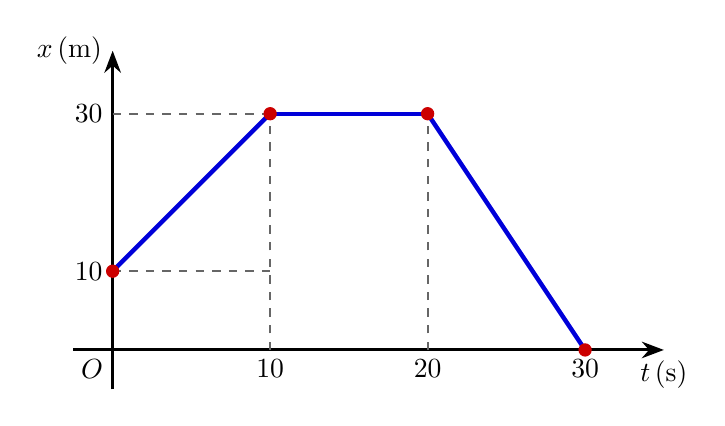
\begin{tikzpicture}[>=Stealth, scale=1.0]
    % محورها
    \draw[->, line width=1.1pt] (-0.5,0) -- (7,0) node[below] {$t\,(\text{s})$};
    \draw[->, line width=1.1pt] (0,-0.5) -- (0,3.8) node[left] {$x\,(\text{m})$};
    \node[below left] at (0,0) {$O$};

    % خطوط راهنما
    \draw[dashed, line width=0.7pt, gray!80!black] (0,3) node[left, black] {$30$} -- (4,3);
    \draw[dashed, line width=0.7pt, gray!80!black] (0,1) node[left, black] {$10$} -- (2,1);
    \draw[dashed, line width=0.7pt, gray!80!black] (2,0) node[below, black] {$10$} -- (2,3);
    \draw[dashed, line width=0.7pt, gray!80!black] (4,0) node[below, black] {$20$} -- (4,3);
    \draw[dashed, line width=0.7pt, gray!80!black] (6,0) node[below, black] {$30$} -- (6,0);

    % نمودار چندبخشی
    \draw[line width=1.6pt, blue!85!black] (0,1) -- (2,3);
    \draw[line width=1.6pt, blue!85!black] (2,3) -- (4,3);
    \draw[line width=1.6pt, blue!85!black] (4,3) -- (6,0);

    % نقاط کلیدی
    \filldraw[red!80!black] (0,1) circle (2.2pt);
    \filldraw[red!80!black] (2,3) circle (2.2pt);
    \filldraw[red!80!black] (4,3) circle (2.2pt);
    \filldraw[red!80!black] (6,0) circle (2.2pt);
\end{tikzpicture}
\end{center}

به پرسش‌های زیر پاسخ دهید:
\begin{enumerate}
    \item[الف)] جهت حرکت موتورسوار را در هر یک از سه بازهٔ زمانی مشخص کنید.
    \item[ب)] سرعت متوسط موتورسوار را در کل بازهٔ زمانی $0$ تا $30\,\text{s}$ به دست آورید.
    \item[پ)] مسافت پیموده‌شده و جابه‌جایی موتورسوار در همین بازهٔ زمانی چقدر است؟
    \item[ت)] تندی متوسط موتورسوار را بیابید و نتیجه را با اندازهٔ سرعت متوسط قسمت «ب» مقایسه کنید.
\end{enumerate}
\end{exambox}

\begin{answerbox}{پاسخ تشریحی مثال ۱}

\begin{itemize}
    \item[الف)] \textbf{جهت حرکت در هر بازه:}
    \begin{itemize}
        \item بازهٔ $[0, 10\,\text{s}]$: نمودار صعودی است (شیب مثبت)؛ پس موتورسوار در \textbf{جهت مثبت} محور $x$ حرکت می‌کند.
        \item بازهٔ $[10\,\text{s}, 20\,\text{s}]$: نمودار افقی است؛ موتورسوار \textbf{ساکن} است.
        \item بازهٔ $[20\,\text{s}, 30\,\text{s}]$: نمودار نزولی است (شیب منفی)؛ پس موتورسوار در \textbf{جهت منفی} محور $x$ حرکت می‌کند.
    \end{itemize}

    \item[ب)] \textbf{سرعت متوسط در کل بازه:} مکان ابتدا و انتهای حرکت را از نمودار می‌خوانیم ($x(0)=10\,\text{m}$ و $x(30)=0$):
    \[
    v_{av} = \frac{x_2 - x_1}{t_2 - t_1} = \frac{0 - 10}{30 - 0} = -\frac{1}{3}\,\frac{\text{m}}{\text{s}} \approx -0.33\,\frac{\text{m}}{\text{s}}
    \]
    علامت منفی نشان می‌دهد که در مجموع، موتورسوار در جهت منفی محور $x$ جابه‌جا شده است.

    \item[پ)] \textbf{مسافت و جابه‌جایی:} چون موتورسوار یک بار تغییر جهت داده است، مسافت با اندازهٔ جابه‌جایی برابر نیست. هر مرحله را جداگانه محاسبه می‌کنیم:
    \[
    \ell_1 = |30-10| = 20\,\text{m} \quad , \quad \ell_2 = 0 \quad , \quad \ell_3 = |0-30| = 30\,\text{m}
    \]
    \[
    \ell = \ell_1 + \ell_2 + \ell_3 = 20 + 0 + 30 = 50\,\text{m}
    \]
    \[
    \Delta x = x(30) - x(0) = 0 - 10 = -10\,\text{m}
    \]

    \item[ت)] \textbf{تندی متوسط:}
    \[
    s_{av} = \frac{\ell}{\Delta t} = \frac{50}{30} = \frac{5}{3}\,\frac{\text{m}}{\text{s}} \approx 1.67\,\frac{\text{m}}{\text{s}}
    \]
    مشاهده می‌شود که $s_{av} > |v_{av}|$؛ زیرا موتورسوار در میانهٔ راه تغییر جهت داده و در نتیجه مسافت پیموده‌شده از اندازهٔ جابه‌جایی بیشتر شده است.
\end{itemize}
\end{answerbox}

% =========================================================================
% بخش ۳: حرکت با سرعت ثابت (بخش ۱-۲ کتاب)
% =========================================================================
\section{حرکت با سرعت ثابت (بخش ۱-۲ کتاب)}

ساده‌ترین نوع حرکت، حرکت با سرعت ثابت است. در این نوع حرکت، اندازه و جهت سرعت متحرک در طول مسیر ثابت است. در چنین حرکتی، شیب نمودار مکان-زمان در تمام طول حرکت ثابت بوده و در نتیجه، سرعت متوسط متحرک در هر بازهٔ زمانی دلخواه، برابر سرعت لحظه‌ای آن است. به این ترتیب می‌توان نوشت:
\[
v_{av} = \frac{\Delta x}{\Delta t} = v \quad \Longrightarrow \quad \Delta x = v\,\Delta t
\]
حالا اگر مطابق تعریف جابه‌جایی، $\Delta x = x - x_0$ و $\Delta t = t - 0$ باشد، رابطهٔ آخر را می‌توان به صورت زیر بازنویسی کرد:

\begin{conceptbox}{معادلهٔ مکان-زمان در حرکت با سرعت ثابت}
\[
x = vt + x_0 \qquad \text{\rl{(معادلهٔ ۱-۴ کتاب)}}
\]
در این معادله، $x_0$ \textbf{مکان اولیه} متحرک؛ یعنی مکان متحرک در لحظهٔ $t=0$ است. توجه کنید که $x_0$ و $x$ به دلیل ماهیت برداری مکان، می‌توانند مثبت، منفی یا صفر باشند. سرعت متحرک نیز در صورتی که حرکت در جهت مثبت محور $x$ باشد مثبت و در غیر این صورت منفی است.
\end{conceptbox}

\begin{tipbox}{ساخت معادلهٔ مکان-زمان از روی نمودار خطی}
هرگاه نمودار مکان-زمان متحرکی خط راست باشد، حرکت آن با سرعت ثابت است و معادلهٔ آن را می‌توان به این صورت نوشت:
\begin{itemize}
    \item \textbf{$x_0$:} عرض از مبدأ نمودار (محل تقاطع نمودار با محور قائم).
    \item \textbf{$v$:} شیب نمودار که از دو نقطهٔ دلخواه روی خط به دست می‌آید:
    \[
    v = \frac{x_2 - x_1}{t_2 - t_1}
    \]
\end{itemize}
برعکس نیز، از روی معادله می‌توان نمودار را رسم کرد: نقطهٔ $(0, x_0)$ را مشخص کرده و با شیب $v$ خط را رسم می‌کنیم.
\end{tipbox}

\begin{exambox}{مثال ۲: تحلیل معادلهٔ مکان-زمان حرکت یکنواخت (نهایی خرداد ۹۹)}
معادلهٔ مکان-زمان متحرکی که روی خط راست و در راستای محور $x$ حرکت می‌کند، به صورت $x = -4t + 6$ است (برحسب SI).
\begin{enumerate}
    \item[الف)] مکان اولیه و سرعت متحرک را به دست آورید و جهت حرکت آن را مشخص کنید.
    \item[ب)] متحرک در چه لحظه‌ای از مبدأ مکان ($x=0$) می‌گذرد؟
    \item[پ)] با تهیهٔ جدول مکان-زمان برای لحظه‌های $t=0$ و $t=3\,\text{s}$، نمودار مکان-زمان متحرک را رسم کنید.
\end{enumerate}
\end{exambox}

\begin{answerbox}{پاسخ تشریحی مثال ۲}
مقایسهٔ معادلهٔ داده‌شده با معادلهٔ ۱-۴ ($x = vt + x_0$) کافی است:
\[
x_0 = +6\,\text{m} \qquad , \qquad v = -4\,\frac{\text{m}}{\text{s}}
\]
\begin{itemize}
    \item[الف)] علامت منفی سرعت نشان می‌دهد که متحرک در \textbf{جهت منفی} محور $x$ حرکت می‌کند. چون سرعت ثابت است، جهت حرکت در تمام طول حرکت همان جهت منفی و بدون تغییر باقی می‌ماند.
    \item[ب)] مکان متحرک را صفر قرار می‌دهیم:
    \[
    0 = -4t + 6 \quad \Longrightarrow \quad t = 1.5\,\text{s}
    \]
    \item[پ)] با جای‌گذاری لحظه‌های خواسته‌شده در معادله:
    \[
    x(0) = +6\,\text{m} \qquad , \qquad x(3) = -4(3) + 6 = -6\,\text{m}
    \]
    نمودار مکان-زمان، خط راستی است که از نقاط $(0, +6)$ و $(3, -6)$ می‌گذرد:
\end{itemize}

\begin{center}
\begin{tikzpicture}[>=Stealth, scale=0.9]
    % محورها
    \draw[->, line width=1.1pt] (-0.5,0) -- (4.4,0) node[below] {$t\,(\text{s})$};
    \draw[->, line width=1.1pt] (0,-2) -- (0,2.2) node[left] {$x\,(\text{m})$};
    \node[below left] at (0,0) {$O$};

    % خطوط راهنما
    \draw[dashed, line width=0.7pt, gray!80!black] (0,1.5) node[left, black] {\small $+6$} -- (0,1.5);
    \draw[dashed, line width=0.7pt, gray!80!black] (0,-1.5) node[left, black] {\small $-6$} -- (3.6,-1.5);
    \draw[dashed, line width=0.7pt, gray!80!black] (1.8,0) node[below, black] {\small $1.5$} -- (1.8,1.5);
    \draw[dashed, line width=0.7pt, gray!80!black] (3.6,0) node[below, black] {\small $3$} -- (3.6,-1.5);

    % نمودار خطی
    \draw[line width=1.6pt, blue!85!black] (0,1.5) -- (3.6,-1.5);

    % نقاط کلیدی
    \filldraw[red!80!black] (0,1.5) circle (2.2pt);
    \filldraw[purple] (1.8,0) circle (2.4pt);
    \node[above right=1pt, purple] at (1.8,0) {\small\rl{عبور از مبدأ}};
    \filldraw[red!80!black] (3.6,-1.5) circle (2.2pt);
\end{tikzpicture}
\end{center}

نمودار دقیقاً در لحظهٔ $t = 1.5\,\text{s}$ محور زمان را قطع می‌کند؛ همان لحظهٔ عبور از مبدأ مکان که در قسمت «ب» به دست آوردیم.
\end{answerbox}

\subsection{دیدار دو متحرک با سرعت ثابت}

از پرتکرارترین سوالات امتحان نهایی، تعیین زمان و مکان دیدار (تقاطع) دو متحرکی است که با سرعت ثابت روی یک خط حرکت می‌کنند. راه‌حل استاندارد این مسئله، \textbf{برابر قرار دادن معادلات مکان-زمان دو متحرک} است؛ زیرا در لحظهٔ دیدار، هر دو در مکان یکسانی قرار دارند. روش دوم، حل گرافیکی مسئله است: محل تقاطع دو خط در نمودار مکان-زمان، زمان و مکان دیدار را نشان می‌دهد.

\begin{exambox}{مثال ۳: دیدار دو کفش دوزک}
دو کفش دوزک که در راستای محور $x$ حرکت می‌کنند، در لحظهٔ $t=0$ در مکان‌های $x_A = 10\,\text{m}$ و $x_B = 70\,\text{m}$ قرار دارند. کفش دوزک اول با سرعت ثابت $+5\,\text{m/s}$ و دومی با سرعت ثابت $-5\,\text{m/s}$ حرکت می‌کنند.

\begin{enumerate}
    \item[الف)] معادلهٔ مکان-زمان هر کفش دوزک را بنویسید.
    \item[ب)] تعیین کنید کفش دوزک‌ها در چه لحظه‌ای و در چه مکانی به یکدیگر می‌رسند.
    \item[پ)] نمودار مکان-زمان هر دو را در یک دستگاه مختصات رسم کرده و نقطهٔ تقاطع را تفسیر کنید.
\end{enumerate}
\end{exambox}

\begin{answerbox}{پاسخ تشریحی مثال ۳}

\begin{itemize}
    \item[الف)] با جای‌گذاری مقادیر $x_0$ و $v$ در معادلهٔ ۱-۴:
    \[
    x_A = 5t + 10 \qquad , \qquad x_B = -5t + 70 \qquad \text{\rl{(برحسب SI)}}
    \]

    \item[ب)] در لحظهٔ دیدار $x_A = x_B$ است؛ پس دو معادله را برابر هم قرار می‌دهیم:
    \[
    5t + 10 = -5t + 70 \quad \Longrightarrow \quad 10t = 60 \quad \Longrightarrow \quad t = 6\,\text{s}
    \]
    با جای‌گذاری این زمان در هر یک از دو معادله:
    \[
    x_A = 5(6) + 10 = 40\,\text{m} \qquad , \qquad x_B = -5(6) + 70 = 40\,\text{m}
    \]
    بنابراین دو کفش دوزک پس از $6\,\text{s}$ در مکان $x = 40\,\text{m}$ به یکدیگر می‌رسند.

    \item[پ)] نمودار هر دو متحرک خط راست است؛ یکی با عرض از مبدأ $10$ و شیب مثبت و دیگری با عرض از مبدأ $70$ و شیب منفی:
\end{itemize}

\begin{center}
\begin{tikzpicture}[>=Stealth, scale=0.95]
    % محورها
    \draw[->, line width=1.1pt] (-0.4,0) -- (7.2,0) node[below] {$t\,(\text{s})$};
    \draw[->, line width=1.1pt] (0,-0.4) -- (0,4.2) node[left] {$x\,(\text{m})$};
    \node[below left] at (0,0) {$O$};

    % خطوط راهنمای مقادیر محورها
    \foreach \y/\l in {0.5/{10}, 2/{40}, 3.5/{70}} {
        \node[left, black] at (0,\y) {\small \l};
    }
    \node[below, black] at (3,0) {\small $6$};
    \node[below, black] at (6,0) {\small $12$};

    % خطوط حرکت دو متحرک
    \draw[line width=1.5pt, blue!85!black] (0,0.5) -- (6,3.5) node[right, black] {$A$};
    \draw[line width=1.5pt, red!80!black] (0,3.5) -- (6,0.5) node[right, black] {$B$};

    % نقطه دیدار
    \draw[dashed, line width=0.7pt, gray!80!black] (0,2) -- (3,2) -- (3,0);
    \filldraw[purple] (3,2) circle (2.6pt);
    \node[above right=2pt, purple] at (3,2) {\small\rl{دیدار}};
\end{tikzpicture}
\end{center}

محل تقاطع دو خط دقیقاً همان نقطهٔ $(6\,\text{s}, 40\,\text{m})$ است که در قسمت «ب» به دست آوردیم؛ یعنی لحظه و مکان دیدار دو متحرک.
\end{answerbox}

\begin{conceptbox}{روش تندی نسبی: راه سریع حل مسائل دیدار و سبقت}
در مسائلی که دو متحرک با سرعت ثابت حرکت می‌کنند، به جای نوشتن دو معادلهٔ مکان-زمان، می‌توانیم خود را جای یکی از متحرک‌ها بگذاریم؛ در این نگاه «نسبی»، آن متحرک ساکن به نظر می‌رسد و دیگری با سرعتی معادل جمع یا اختلاف دو سرعت حرکت می‌کند. اگر فاصلهٔ اولیهٔ دو متحرک $D$ باشد، زمان دیدار از روابط زیر به دست می‌آید:
\begin{itemize}
    \item \textbf{حرکت به سمت یکدیگر (مخالف‌جهت):} در هر ثانیه فاصلهٔ میان آن‌ها به اندازهٔ مجموع تندی‌ها کم می‌شود:
    \[
    t_{\text{\rl{دیدار}}} = \frac{D}{|v_A| + |v_B|}
    \]
    \item \textbf{تعقیب و سبقت (هم‌جهت):} متحرک عقب‌تر فقط وقتی می‌تواند به جلوتر برسد که تندتر باشد ($|v_A| > |v_B|$)؛ در هر ثانیه، فاصله به اندازهٔ اختلاف تندی‌ها کم می‌شود:
    \[
    t_{\text{\rl{رسیدن}}} = \frac{D}{|v_A| - |v_B|}
    \]
\end{itemize}
\textbf{وارسی روی مثال ۳:} فاصلهٔ اولیهٔ دو کفش دوزک برابر $D = 70 - 10 = 60\,\text{m}$ بود و چون به سمت یکدیگر حرکت می‌کردند:
\[
t = \frac{D}{|v_A| + |v_B|} = \frac{60}{5 + 5} = 6\,\text{s}
\]
که دقیقاً همان پاسخ قسمت «ب» است. توجه کنید که این روش تنها برای سرعت‌های ثابت معتبر است؛ اما به دلیل سادگی، در آزمون‌های تستی بسیار کارآمد می‌باشد.
\end{conceptbox}

% =========================================================================
% بخش ۴: حرکت با شتاب ثابت (بخش ۱-۳ کتاب)
% =========================================================================
\section{حرکت با شتاب ثابت (بخش ۱-۳ کتاب)}

در بخش قبل دیدیم که هرگاه سرعت جسمی تغییر کند، آن جسم شتاب دارد. تغییر سرعت می‌تواند به دلیل تغییر در اندازهٔ سرعت، تغییر در جهت سرعت، یا هر دو باشد. در این بخش به بررسی مهم‌ترین نوع حرکت شتاب‌دار، یعنی \textbf{حرکت با شتاب ثابت} می‌پردازیم.

\subsection{شتاب متوسط و شتاب لحظه‌ای}

\begin{conceptbox}{تعریف شتاب متوسط}
شتاب متوسط متحرک در هر بازهٔ زمانی دلخواه $t_1$ تا $t_2$ به صورت نسبت تغییر سرعت به مدت زمان آن بازه تعریف می‌شود:
\[
\vec{a}_{av} = \frac{\Delta\vec{v}}{\Delta t} = \frac{\vec{v}_2 - \vec{v}_1}{t_2 - t_1} \qquad \text{\rl{(رابطهٔ ۱-۵ کتاب)}}
\]
شتاب کمیتی \textbf{برداری} است و جهت آن همواره با بردار \textbf{تغییر سرعت} ($\Delta\vec{v}$) یکی است. یکای شتاب در SI متر بر مجذور ثانیه ($\text{m/s}^2$) است.
\end{conceptbox}

چون در این کتاب تنها حرکت روی خط راست بررسی می‌شود، می‌توان به جای عملیات برداری، از مؤلفه‌های علامت‌دار سرعت استفاده کرد:

\begin{conceptbox}{شتاب متوسط در راستای محور $x$}
\[
a_{av} = \frac{v_2 - v_1}{t_2 - t_1} \qquad \text{\rl{(رابطهٔ ۱-۶ کتاب)}}
\]
هنگام استفاده از این رابطه باید به علامت سرعت‌ها که نشان‌دهندهٔ جهت آنهاست، توجه کنیم.
\end{conceptbox}

مشابه آنچه برای سرعت دیدیم، اگر در رابطهٔ شتاب متوسط، $\Delta t$ را به سمت صفر میل دهیم، به مفهوم \textbf{شتاب لحظه‌ای} می‌رسیم: شتاب در هر لحظهٔ دلخواه، برابر شیب خط مماس بر نمودار سرعت-زمان در آن لحظه است. برای سادگی، در سراسر این کتاب شتاب لحظه‌ای را به اختصار «شتاب» می‌نامیم و آن را با نماد $a$ نشان می‌دهیم.

\subsection{تعریف حرکت با شتاب ثابت}

هرگاه شتاب متحرک در لحظه‌های مختلف یکسان باشد؛ یعنی در هر بازهٔ زمانی دلخواه، شتاب متوسط برابر شتاب لحظه‌ای باشد، حرکت جسم را \textbf{حرکت با شتاب ثابت} می‌نامیم. در چنین حرکتی، نمودار سرعت-زمان خطی است و شیب آن در تمام طول حرکت یکسان است. حرکت اجسامی مانند جسمی که روی سطح هموار یک سراشیبی می‌لغزد، خودرویی که پس از سبز شدن چراغ راهنمایی حرکت می‌کند، یا هواپیمایی که روی باند پرواز حرکت می‌کند تا به شرایط لازم برای برخاستن برسد، تقریباً با شتاب ثابت است.

\begin{center}
\begin{tikzpicture}[>=Stealth, scale=0.9]
    % محورها
    \draw[->, line width=1.1pt] (-0.4,0) -- (5.2,0) node[below] {$t$};
    \draw[->, line width=1.1pt] (0,-0.4) -- (0,3.6) node[left] {$v$};

    % خط سرعت-زمان
    \draw[line width=1.5pt, blue!85!black] (0,1) -- (4.2,3.1);
    \draw[dashed, line width=0.7pt, gray!80!black] (0,1) node[left, black] {\small $v_0$} -- (0,0);
    \draw[dashed, line width=0.7pt, gray!80!black] (4.2,3.1) -- (4.2,0) node[below, black] {\small $t$};
    \draw[dashed, line width=0.7pt, gray!80!black] (4.2,3.1) -- (0,3.1) node[left, black] {\small $v$};

    % نمایش شیب
    \draw[line width=1pt, orange!90!black] (1.2,1.57) -- (2.2,2.07);
    \draw[line width=1pt, orange!90!black] (1.2,1.57) -- (2.2,1.57);
    \node[orange!90!black, below right] at (1.35,1.55) {\small $\Delta t$};
    \node[orange!90!black, right] at (2.25,1.82) {\small $\Delta v$};
    \node[blue!85!black, above left] at (2.6,2.45) {\small\lr{$= a$} \rl{شیب}};
\end{tikzpicture}
\end{center}

\subsection{چهار معادلهٔ طلایی حرکت با شتاب ثابت}

اگر سرعت متحرک در لحظهٔ $t=0$ برابر $v_0$ (سرعت اولیه) و در لحظهٔ $t$ برابر $v$ باشد، از تعریف شتاب ثابت ($a = a_{av}$) معادلات حرکت به دست می‌آیند. این چهار معادله، ابزار اصلی حل مسائل این فصل و پرتکرارترین روابط سوالات کنکور هستند:

\begin{conceptbox}{معادلات حرکت با شتاب ثابت}
\begin{enumerate}
    \item \textbf{سرعت-زمان:}
    \[
    v = at + v_0 \qquad \text{\rl{(معادلهٔ ۱-۸ کتاب)}}
    \]
    \item \textbf{سرعت متوسط (فقط در حرکت با شتاب ثابت):}
    \[
    v_{av} = \frac{v + v_0}{2} \qquad \text{\rl{(معادلهٔ ۱-۹ کتاب)}}
    \]
    \item \textbf{مکان-زمان:}
    \[
    x = \frac{1}{2}at^2 + v_0 t + x_0 \qquad \text{\rl{(معادلهٔ ۱-۱۰ کتاب)}}
    \]
    \item \textbf{سرعت-جابه‌جایی:}
    \[
    v^2 = v_0^2 + 2a\,\Delta x \qquad \text{\rl{(معادلهٔ ۱-۱۱ کتاب)}}
    \]
\end{enumerate}
توجه کنید که معادلهٔ ۱-۹ را برای هر بازهٔ زمانی دلخواه نیز می‌توان به کار برد؛ به شرط آنکه شتاب در آن بازه ثابت باشد:
\[
v_{av} = \frac{v_1 + v_2}{2}
\]
\end{conceptbox}

\begin{tipbox}{جدول انتخاب معادله - کدام معادله کجا؟}
راهبرد حل مسئله: ابتدا کمیت‌های داده‌شده و کمیت خواسته‌شده را فهرست کنید؛ سپس معادله‌ای را به کار ببرید که \textbf{کمیت ناشناختهٔ سوم} در آن ظاهر نشود:
\begin{center}
\begin{tabular}{p{2.2cm} p{4.6cm} p{2.6cm} p{4.2cm}}
\toprule
\textbf{معادله} & \textbf{رابطه} & \textbf{کمیت غایب} & \textbf{بهترین کاربرد} \\
\midrule
۱-۸ & $v = at + v_0$ & جابه‌جایی & یافتن سرعت یا زمان \\
۱-۹ & $v_{av} = \dfrac{v+v_0}{2}$ & شتاب & محاسبهٔ سریع سرعت متوسط \\
ترکیب ۱-۹ با تعریف & $\Delta x = \dfrac{v_1+v_2}{2}\,t$ & شتاب & محاسبهٔ مستقیم جابه‌جایی از دو سرعت و زمان \\
۱-۱۰ & $x = x_0 + v_0 t + \dfrac{1}{2}at^2$ & سرعت & یافتن مکان یا زمان \\
۱-۱۱ & $v^2 = v_0^2 + 2a\,\Delta x$ & زمان & مسائلی که زمان داده نشده است \\
\bottomrule
\end{tabular}
\end{center}
\end{tipbox}

\begin{tipbox}{معادلهٔ پنجم (بدون سرعت اولیه) - فراتر از کتاب درسی}
اگر رابطهٔ $v_0 = v - at$ را که از معادلهٔ ۱-۸ به دست می‌آید، در معادلهٔ ۱-۱۰ جای‌گذاری کنیم، سرعت اولیه حذف شده و به معادله‌ای می‌رسیم که در آن فقط $v$ (سرعت پایان بازه) ظاهر می‌شود:
\[
\Delta x = v\,t - \frac{1}{2}a\,t^2
\]
این معادله در شماره‌گذاری کتاب درسی نیامده است، اما هنگامی کاربرد دارد که سرعت پایانی و مدت زمان حرکت داده شده باشند و سرعت اولیه مجهول باشد. دقت کنید که این رابطه جدید نیست و صرفاً ترکیبی از معادلات قبلی است.
\end{tipbox}

\begin{exambox}{مثال ۴: یافتن شتاب و زمان از دو حالت معلوم (نهایی شهریور ۹۹)}
متحرکی روی خط راست با شتاب ثابت در راستای محور $x$ حرکت می‌کند. هنگامی که متحرک در مکان $x_1 = 10\,\text{m}$ است، سرعت آن $4\,\text{m/s}$ و هنگامی که به مکان $x_2 = 20\,\text{m}$ می‌رسد، سرعت آن $6\,\text{m/s}$ است.
\begin{enumerate}
    \item[الف)] شتاب متحرک را به دست آورید.
    \item[ب)] مدت زمان حرکت میان این دو مکان چقدر است؟
    \item[پ)] در این بازه، حرکت متحرک تندشونده است یا کندشونده؟
\end{enumerate}
\end{exambox}

\begin{answerbox}{پاسخ تشریحی مثال ۴}
داده‌ها: $v_1 = +4\,\frac{\text{m}}{\text{s}}$، $v_2 = +6\,\frac{\text{m}}{\text{s}}$ و $\Delta x = x_2 - x_1 = 10\,\text{m}$. توجه کنید که زمان در هیچ‌کدام از داده‌ها ظاهر نشده است.

\begin{itemize}
    \item[الف)] چون زمان مجهول است، از معادلهٔ ۱-۱۱ (مستقل از زمان) استفاده می‌کنیم:
    \[
    v_2^2 = v_1^2 + 2a\,\Delta x \quad \Longrightarrow \quad (6)^2 = (4)^2 + 2a(10) \quad \Longrightarrow \quad 20a = 20 \quad \Longrightarrow \quad a = +1\,\frac{\text{m}}{\text{s}^2}
    \]
    \item[ب)] این بار شتاب مجهول است؛ پس ترکیب معادلهٔ ۱-۹ با تعریف سرعت متوسط (معادلهٔ مستقل از شتاب) کارساز است:
    \[
    \Delta x = \frac{v_1 + v_2}{2}\,t \quad \Longrightarrow \quad 10 = \frac{6+4}{2}\,t \quad \Longrightarrow \quad t = 2\,\text{s}
    \]
    \item[پ)] سرعت و شتاب هر دو مثبت‌اند؛ پس هم‌جهت‌اند و حرکت \textbf{تندشونده} است. این نتیجه با محاسبات نیز سازگار است: سرعت متحرک از $4$ به $6\,\text{m/s}$ افزایش یافته است.
\end{itemize}
\end{answerbox}

\subsection{تحلیل هندسی سهمی نمودار مکان-زمان}

در حرکت با شتاب ثابت، معادلهٔ مکان-زمان (معادلهٔ ۱-۱۰) یک تابع درجه دوم از زمان است؛ بنابراین نمودار مکان-زمان همواره یک \textbf{سهمی} است. شکل این سهمی، اطلاعات فیزیکی مهمی دربارهٔ حرکت متحرک در اختیار ما قرار می‌دهد:

\begin{conceptbox}{جهت تقعر سهمی و رأس آن}
\begin{itemize}
    \item \textbf{جهت تقعر، نشانگر علامت شتاب است.} ضریب جملهٔ $t^2$ در معادلهٔ مکان-زمان برابر $\frac{1}{2}a$ است؛ پس:
    \begin{itemize}
        \item اگر $a > 0$ باشد، سهمی \textbf{تقعر رو به بالا} ($\cup$) دارد.
        \item اگر $a < 0$ باشد، سهمی \textbf{تقعر رو به پایین} ($\cap$) دارد.
    \end{itemize}
    توجه کنید که جهت تقعر فقط به علامت شتاب بستگی دارد و علامت سرعت اولیه در آن نقشی ندارد.
    \item \textbf{رأس سهمی، لحظهٔ توقف و تغییر جهت است.} شیب نمودار در رأس صفر است؛ یعنی سرعت لحظه‌ای آنجا صفر بوده و متحرک برای یک لحظه می‌ایستد و جهت خود را عوض می‌کند. لحظهٔ رأس را از صفر گذاشتن معادلهٔ ۱-۸ به دست می‌آوریم:
    \[
    v = at + v_0 = 0
    \qquad \Longrightarrow \qquad
    t_{\text{\rl{رأس}}} = -\frac{v_0}{a}
    \]
    این لحظه تنها زمانی در آینده ($t > 0$) اتفاق می‌افتد که $v_0$ و $a$ \textbf{علامت مخالف} داشته باشند. اگر $v_0$ و $a$ هم‌علامت باشند، رأس سهمی در گذشتهٔ زمانی قرار دارد و متحرک هیچ‌گاه تغییر جهت نمی‌دهد.
\end{itemize}
\end{conceptbox}

\begin{center}
\begin{tikzpicture}[>=Stealth, scale=1.0]
    % ---------- سهمی با تقعر رو به بالا ----------
    \begin{scope}
        \draw[->, line width=1.1pt] (-0.3,0) -- (4.6,0) node[below] {$t$};
        \draw[->, line width=1.1pt] (0,-0.6) -- (0,4.3) node[left] {$x$};
        \node[below left] at (0,0) {$O$};

        % عنوان نمودار
        \node[font=\bfseries\titlefont] at (2.3,4.05) {\rl{تقعر رو به بالا} \lr{($a>0$)}};

        % سهمی
        \draw[domain=0.2:4.3, smooth, variable=\t, line width=1.4pt, blue!85!black]
            plot ({\t}, {0.55*(\t-2.2)*(\t-2.2) + 0.45});

        % رأس و مماس افقی
        \draw[line width=1pt, orange!90!black] (1.2,0.45) -- (3.2,0.45);
        \filldraw[red!80!black] (2.2,0.45) circle (2.2pt);
        \draw[dashed, line width=0.7pt, gray!80!black] (2.2,0) node[below, black] {$t_{\text{\rl{رأس}}}$} -- (2.2,0.45);
        \node[right=2pt] at (3.25,0.45) {\footnotesize\lr{$v=0$} \rl{مماس افقی:}};
    \end{scope}

    % ---------- سهمی با تقعر رو به پایین ----------
    \begin{scope}[xshift=7.2cm]
        \draw[->, line width=1.1pt] (-0.3,0) -- (4.6,0) node[below] {$t$};
        \draw[->, line width=1.1pt] (0,-0.6) -- (0,4.3) node[left] {$x$};
        \node[below left] at (0,0) {$O$};

        % عنوان نمودار
        \node[font=\bfseries\titlefont] at (2.3,4.05) {\rl{تقعر رو به پایین} \lr{($a<0$)}};

        % سهمی
        \draw[domain=0.2:4.3, smooth, variable=\t, line width=1.4pt, teal!80!black]
            plot ({\t}, {-0.55*(\t-2.2)*(\t-2.2) + 3.3});

        % قله و مماس افقی
        \draw[line width=1pt, orange!90!black] (1.2,3.3) -- (3.2,3.3);
        \filldraw[red!80!black] (2.2,3.3) circle (2.2pt);
        \draw[dashed, line width=0.7pt, gray!80!black] (2.2,0) node[below, black] {$t_{\text{\rl{رأس}}}$} -- (2.2,3.3);
        \node[below left=1pt] at (1.25,3.28) {\footnotesize\lr{$x_{\max}$، $v=0$}};
    \end{scope}
\end{tikzpicture}
\end{center}

در هر دو نمودار بالا، رأس سهمی همان نقطهٔ بازگشت متحرک است. در نمودار سمت راست ($a>0$)، متحرک نخست کندشونده و در خلاف جهت محور حرکت می‌کند و پس از توقف در رأس، تندشونده و در جهت محور ادامه می‌دهد. در نمودار سمت چپ ($a<0$)، وضعیت برعکس است: متحرک تا رسیدن به بیشینهٔ مکان ($x_{\max}$ در قلهٔ سهمی) کندشونده است و سپس بازمی‌گردد.

\begin{exambox}{مثال ۵: برخاستن هواپیما از باند پرواز}
شکل روبه‌رو، هواپیمایی را نشان می‌دهد که از حال سکون و با شتاب ثابت $2.2\,\text{m/s}^2$ روی باند پرواز، در امتداد محور $x$ شروع به حرکت می‌کند. هواپیما هنگامی آمادهٔ برخاستن است که سرعت آن به $95\,\text{m/s}$ برسد.

\begin{enumerate}
    \item[الف)] چه مدت طول می‌کشد تا هواپیما به شرایط برخاستن برسد؟
    \item[ب)] سرعت متوسط هواپیما در این بازهٔ زمانی چقدر است؟
    \item[پ)] جابه‌جایی هواپیما در این مدت چقدر است؟
\end{enumerate}
\end{exambox}

\begin{answerbox}{پاسخ تشریحی مثال ۵}

با توجه به ثابت بودن شتاب، از معادلات حرکت با شتاب ثابت استفاده می‌کنیم. داده‌ها: $v_0 = 0$، $a = +2.2\,\text{m/s}^2$ و $v = 95\,\text{m/s}$.

\begin{itemize}
    \item[الف)] از معادلهٔ ۱-۸ (که در آن جابه‌جایی غایب است):
    \[
    v = at + v_0 \quad \Longrightarrow \quad 95 = (2.2)t + 0 \quad \Longrightarrow \quad t \approx 43.2\,\text{s}
    \]

    \item[ب)] چون شتاب ثابت است، از معادلهٔ ۱-۹:
    \[
    v_{av} = \frac{v + v_0}{2} = \frac{95 + 0}{2} = 47.5\,\frac{\text{m}}{\text{s}}
    \]

    \item[پ)] از تعریف سرعت متوسط:
    \[
    \Delta x = v_{av}\,\Delta t = (47.5)(43.2) \approx 2052\,\text{m}
    \]
\end{itemize}

همین تحلیل، مبنای طراحی طول باند فرودگاه‌هاست؛ مهندسان باید بدانند هر هواپیما پیش از رسیدن به سرعت برخاستن، چه مسافتی را روی باند طی می‌کند تا باند را به اندازهٔ کافی بلند بسازند.
\end{answerbox}

\subsection{منطق تندشونده و کندشونده بودن حرکت}

\begin{tipbox}{قاعدهٔ طلایی: هم‌جهتی سرعت و شتاب}
واژه‌های «تندشونده» و «کندشونده» به افزایش یا کاهش \textbf{تندی} متحرک اشاره دارند، نه به علامت سرعت. قاعدهٔ تصمیم‌گیری بسیار ساده است:
\begin{center}
\textbf{اگر سرعت و شتاب هم‌جهت باشند، حرکت تندشونده است و اگر خلاف جهت هم باشند، حرکت کندشونده است.}
\end{center}
\begin{center}
\begin{tabular}{c c c c}
\toprule
\textbf{علامت $v$} & \textbf{علامت $a$} & \textbf{وضعیت} & \textbf{نوع حرکت} \\
\midrule
مثبت & مثبت & هم‌جهت & تندشونده \\
منفی & منفی & هم‌جهت & تندشونده \\
مثبت & منفی & خلاف جهت & کندشونده \\
منفی & مثبت & خلاف جهت & کندشونده \\
\bottomrule
\end{tabular}
\end{center}
\textbf{مثال مهم:} خودرویی که در جهت منفی محور $x$ در حال حرکت است و ترمز می‌گیرد، شتاب مثبت دارد؛ اما چون سرعت و شتاب خلاف جهت یکدیگرند، حرکت آن \textbf{کندشونده} است. فراموش نکنید که در لحظه‌ای که سرعت صفر می‌شود ($v=0$)، جهت حرکت ممکن است تغییر کند.
\end{tipbox}

\subsection{مساحت زیر نمودار سرعت-زمان}

نتیجهٔ بسیار مهمی که در حل مسائل کاربرد فراوان دارد این است که:

\begin{conceptbox}{مساحت زیر نمودار $v$-$t$ برابر جابه‌جایی است}
مساحت ناحیهٔ بین نمودار سرعت-زمان و محور زمان، برابر \textbf{جابه‌جایی} متحرک است. دو نکتهٔ اساسی:
\begin{itemize}
    \item نواحی که بالای محور زمان قرار دارند، مثبت و نواحی زیر محور زمان، منفی حساب می‌شوند.
    \item \textbf{مسافت پیموده‌شده} برابر مجموع قدرمطلق مساحت‌های همهٔ نواحی است.
\end{itemize}
\end{conceptbox}

\begin{exambox}{مثال ۶: جابه‌جایی و مسافت از روی مساحت زیر نمودار $v$-$t$}
متحرکی که در راستای محور $x$ حرکت می‌کند، از مکان $x_0 = 0$ حرکت خود را آغاز کرده است. نمودار سرعت-زمان این متحرک مطابق شکل زیر است:

\begin{center}
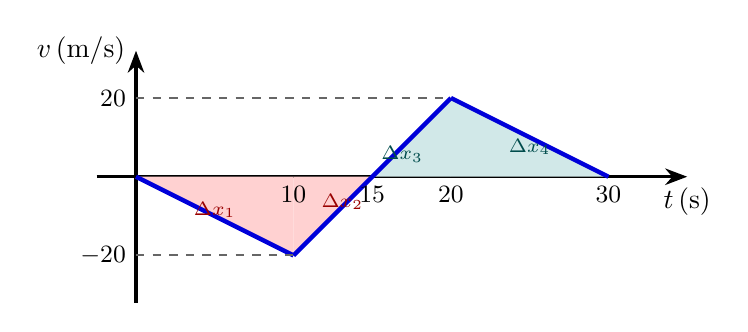
\begin{tikzpicture}[>=Stealth, scale=1.0]
    % محورها
    \draw[->, line width=1.1pt] (-0.5,0) -- (7,0) node[below] {$t\,(\text{s})$};
    \draw[->, line width=1.1pt] (0,-1.6) -- (0,1.6) node[left] {$v\,(\text{m/s})$};

    % نواحی سایه‌دار
    \fill[red!18] (0,0) -- (2,-1) -- (2,0) -- cycle;
    \fill[red!18] (2,0) -- (3,0) -- (2,-1) -- cycle;
    \fill[teal!18] (3,0) -- (4,0) -- (4,1) -- cycle;
    \fill[teal!18] (4,1) -- (4,0) -- (6,0) -- cycle;

    % نمودار
    \draw[line width=1.6pt, blue!85!black] (0,0) -- (2,-1);
    \draw[line width=1.6pt, blue!85!black] (2,-1) -- (4,1);
    \draw[line width=1.6pt, blue!85!black] (4,1) -- (6,0);

    % خطوط راهنما
    \draw[dashed, line width=0.7pt, gray!80!black] (0,-1) node[left, black] {\small $-20$} -- (2,-1);
    \draw[dashed, line width=0.7pt, gray!80!black] (0,1) node[left, black] {\small $20$} -- (4,1);
    \foreach \x/\l in {2/{10}, 3/{15}, 4/{20}, 6/{30}} {
        \node[below, black] at (\x,0) {\small \l};
    }

    % برچسب نواحی
    \node[red!60!black] at (1,-0.42) {\scriptsize $\Delta x_1$};
    \node[red!60!black] at (2.62,-0.32) {\scriptsize $\Delta x_2$};
    \node[teal!60!black] at (3.38,0.28) {\scriptsize $\Delta x_3$};
    \node[teal!60!black] at (5,0.38) {\scriptsize $\Delta x_4$};
\end{tikzpicture}
\end{center}

\begin{enumerate}
    \item[الف)] جابه‌جایی و مسافت پیموده‌شدهٔ متحرک در کل زمان حرکت ($30\,\text{s}$) را بیابید.
    \item[ب)] در کدام لحظه جهت حرکت متحرک تغییر کرده است؟
    \item[پ)] نوع حرکت (تندشونده یا کندشونده) را در هر بازه مشخص کنید.
\end{enumerate}
\end{exambox}

\begin{answerbox}{پاسخ تشریحی مثال ۶}

\begin{itemize}
    \item[الف)] مساحت هر ناحیه را جداگانه محاسبه می‌کنیم؛ نواحی بالای محور زمان مثبت و نواحی زیر آن منفی‌اند:
    \[
    \Delta x_1 = \frac{1}{2}(10)(-20) = -100\,\text{m} \qquad , \qquad \Delta x_2 = \frac{1}{2}(5)(-20) = -50\,\text{m}
    \]
    \[
    \Delta x_3 = \frac{1}{2}(5)(+20) = +50\,\text{m} \qquad , \qquad \Delta x_4 = \frac{1}{2}(10)(+20) = +100\,\text{m}
    \]
    بنابراین:
    \[
    \Delta x = \Delta x_1 + \Delta x_2 + \Delta x_3 + \Delta x_4 = -100 - 50 + 50 + 100 = 0
    \]
    \[
    \ell = |\Delta x_1| + |\Delta x_2| + |\Delta x_3| + |\Delta x_4| = 100 + 50 + 50 + 100 = 300\,\text{m}
    \]
    نتیجهٔ جالب: جابه‌جایی متحرک صفر است؛ اما مسافت پیموده‌شده $300\,\text{m}$ است و تندی متوسط آن $s_{av} = \frac{300}{30} = 10\,\text{m/s}$ می‌باشد.

    \item[ب)] جهت حرکت تنها جایی تغییر می‌کند که سرعت از مثبت به منفی (یا برعکس) تغییر علامت دهد؛ یعنی محل تقاطع نمودار با محور زمان: در لحظهٔ $t = 15\,\text{s}$.

    \item[پ)] با مقایسهٔ علامت سرعت و شتاب (شیب نمودار) در هر بازه:
    \begin{itemize}
        \item بازهٔ $[0, 10\,\text{s}]$: $v<0$ و $a<0$ (شیب منفی) $\Leftarrow$ هم‌جهت $\Leftarrow$ \textbf{تندشونده}.
        \item بازهٔ $[10\,\text{s}, 15\,\text{s}]$: $v<0$ و $a>0$ $\Leftarrow$ خلاف جهت $\Leftarrow$ \textbf{کندشونده}.
        \item بازهٔ $[15\,\text{s}, 20\,\text{s}]$: $v>0$ و $a>0$ $\Leftarrow$ هم‌جهت $\Leftarrow$ \textbf{تندشونده}.
        \item بازهٔ $[20\,\text{s}, 30\,\text{s}]$: $v>0$ و $a<0$ $\Leftarrow$ خلاف جهت $\Leftarrow$ \textbf{کندشونده}.
    \end{itemize}
\end{itemize}
\end{answerbox}

\subsection{جابه‌جایی در ثانیه‌های متوالی و الگوی اعداد فرد گالیله}
منظور از «ثانیهٔ $n$‌ام»، بازهٔ زمانی یک‌ثانیه‌ای میان لحظه‌های $(n-1)$ و $n$ است. متحرکی که با شتاب ثابت حرکت می‌کند، در این ثانیه‌های متوالی از الگوهای ساده و زیبایی پیروی می‌کند که حل بسیاری از مسائل را بدون جای‌گذاری طولانی در معادلات اصلی ممکن می‌سازد.

\begin{conceptbox}{الگوی گالیله برای حرکت از حال سکون ($v_0 = 0$)}
اگر متحرکی از حال سکون با شتاب ثابت $a$ حرکت کند، مکان آن از لحظهٔ شروع برابر است با $x = \frac{1}{2}at^2$. از همین رابطهٔ ساده، دو تناسب طلایی به دست می‌آید:
\begin{itemize}
    \item \textbf{مکان از ابتدای حرکت} تا پایان ثانیه‌های متوالی، نسبت مربع کامل دارد:
    \[
    x(1) : x(2) : x(3) : \dots : x(n) = 1 : 4 : 9 : \dots : n^2
    \]
    \item \textbf{جابه‌جایی در ثانیه‌های متوالی،} نسبت اعداد فرد دارد:
    \[
    \Delta x_1 : \Delta x_2 : \Delta x_3 : \dots : \Delta x_n = 1 : 3 : 5 : \dots : (2n-1)
    \]
\end{itemize}
دلیل این الگو آن است که اختلاف مربع‌های متوالی، اعداد فرد را می‌سازد:
\[
\Delta x_n = n^2 - (n-1)^2 = 2n - 1
\]
\end{conceptbox}

\begin{conceptbox}{فرمول کلی جابه‌جایی در ثانیهٔ $n$‌ام (با سرعت اولیه)}
اگر متحرکی با شتاب ثابت، در لحظهٔ $t=0$ حرکت خود را با سرعت اولیهٔ $v_0$ آغاز کند، جابه‌جایی آن در ثانیهٔ $n$‌ام (بازهٔ یک‌ثانیه‌ای) از رابطهٔ زیر به دست می‌آید:
\[
\Delta x_n = x(n) - x(n-1) = \frac{1}{2}a\,(2n-1) + v_0
\]
نکتهٔ کاربردی: اگر جابه‌جایی دو ثانیهٔ دلخواه را از یکدیگر کم کنیم، سرعت اولیه حذف می‌شود:
\[
\Delta x_m - \Delta x_n = a\,(m-n)
\]
این رابطه در مسائلی که «اختلاف جابه‌جایی دو ثانیه» داده شده است، بسیار سریع به شتاب می‌رسد.
\end{conceptbox}

\begin{tipbox}{تعمیم به بازه‌های $T$ ثانیه‌ای (نکتهٔ کنکوری)}
اگر بازه‌های زمانی به‌جای یک ثانیه، هر کدام $T$ ثانیه باشند، همان الگوی تصاعدی با مقیاس جدید برقرار می‌شود؛ جابه‌جایی در بازهٔ $n$‌ام از این بازه‌های متوالی برابر است با:
\[
\Delta x_{T_n} = \left(n - \frac{1}{2}\right)a\,T^2 + v_0\,T
\]
در سقوط آزاد ($a = -g$ و $v_0 = 0$) این رابطه ساده‌تر می‌شود:
\[
\Delta y_{T_n} = -\frac{1}{2}g\,(2n-1)\,T^2
\]
برای نمونه، مسافت سقوط در ثانیهٔ سوم ($T = 1\,\text{s}$ و $n = 3$ با $g = 10\,\text{m/s}^2$) برابر $\frac{1}{2}(10)(5)(1)^2 = 25\,\text{m}$ است؛ همان ستون «مسافت همین ثانیه» در جدول میان‌بر بخش سقوط آزاد.
\end{tipbox}

\begin{tipbox}{تکنیک معکوس زمانی: ترمز تا توقف، قرینهٔ شروع از سکون}
حرکتی را در نظر بگیرید که با شتاب ثابت ترمز می‌گیرد و سرانجام کاملاً متوقف می‌شود. اگر فیلم این حرکت را از آخر به اول تماشا کنیم، حرکتی خواهیم دید که از حال سکون با تندیِ فزاینده آغاز می‌شود؛ یعنی دقیقاً قرینهٔ حرکت گالیله. نتیجهٔ عملی این تقارن چنین است:
\begin{itemize}
    \item جابه‌جایی در \textbf{ثانیهٔ آخر} حرکت ترمز برابر است با:
    \[
    \Delta x_{\text{\rl{آخر}}} = \frac{1}{2}|a| \times (1)^2
    \]
    \item جابه‌جایی در ثانیهٔ قبل از آن $\frac{3}{2}|a|$، و قبل از آن $\frac{5}{2}|a|$ است؛ یعنی همان الگوی اعداد فرد، این بار از انتهای مسیر رو به عقب.
\end{itemize}
\end{tipbox}

\begin{exambox}{مثال ۷: جابه‌جایی خودرو در ثانیهٔ آخر ترمز}
خودرویی با سرعت $108\,\text{km/h}$ در حال حرکت است که راننده ترمز می‌گیرد و خودرو با شتاب ثابت $5\,\text{m/s}^2$ کند می‌شود تا کاملاً متوقف شود. جابه‌جایی خودرو در ثانیهٔ آخر حرکت چند متر است؟
\end{exambox}

\begin{answerbox}{پاسخ تشریحی مثال ۷}

ابتدا یکاها را هماهنگ می‌کنیم و مدت کل ترمزگیری را می‌یابیم:
\[
v_0 = \frac{108}{3.6} = 30\,\frac{\text{m}}{\text{s}}
\qquad , \qquad
t_{\text{\rl{توقف}}} = \frac{v_0}{|a|} = \frac{30}{5} = 6\,\text{s}
\]
پس ثانیهٔ آخر حرکت، بازهٔ میان لحظه‌های $t=5\,\text{s}$ و $t=6\,\text{s}$ است. این جابه‌جایی را به دو روش محاسبه می‌کنیم:

\begin{itemize}
    \item \textbf{روش ۱ (فرمول ثانیهٔ $n$‌ام):} با قرار دادن $a=-5\,\text{m/s}^2$، $v_0=30\,\text{m/s}$ و $n=6$ در فرمول کلی:
    \[
    \Delta x_6 = \frac{1}{2}(-5)(2 \times 6 - 1) + 30 = -27.5 + 30 = 2.5\,\text{m}
    \]

    \item \textbf{روش ۲ (تکنیک معکوس زمانی):} مطابق نکتهٔ بالا، جابه‌جایی ثانیهٔ آخر ترمز با جابه‌جایی ثانیهٔ اول حرکت از سکون برابر است:
    \[
    \Delta x_{\text{\rl{آخر}}} = \frac{1}{2}(5)(1)^2 = 2.5\,\text{m}
    \]
\end{itemize}

هر دو روش پاسخ یکسانی می‌دهند: خودرو در ثانیهٔ آخر تنها $2.5\,\text{m}$ جابه‌جا می‌شود؛ حال آنکه در ثانیهٔ اول ترمز این مقدار $27.5\,\text{m}$ بود. این مقایسه به خوبی نشان می‌دهد که خودرو پیش از توقف، چه اندازه آرام می‌گیرد.
\end{answerbox}

\subsection{کاربرد معادلات در مسائل ترمز و توقف}

\begin{exambox}{مثال ۸: ترمز گرفتن خودرو در برابر گوزن}
خودرویی با سرعت $111\,\text{km/h}$ در یک پارک حفاظت‌شده، در یک راه مستقیم در حال حرکت است که ناگهان گوزنی را در فاصلهٔ $220\,\text{m}$ جلوی خود می‌بیند و بلافاصله ترمز می‌گیرد. حرکت خودرو با شتاب ثابتی به اندازهٔ $3.8\,\text{m/s}^2$ کند می‌شود تا سرانجام متوقف شود.

\begin{enumerate}
    \item[الف)] خودرو در چه فاصله‌ای از محل ترمزگیری متوقف می‌شود؟ آیا با گوزن برخورد می‌کند؟
    \item[ب)] چه مدت طول می‌کشد تا خودرو متوقف شود؟
\end{enumerate}
\end{exambox}

\begin{answerbox}{پاسخ تشریحی مثال ۸}

ابتدا داده‌ها را هماهنگ می‌کنیم. جهت حرکت خودرو را جهت مثبت محور $x$ می‌گیریم و مبدأ را محل ترمزگیری در نظر می‌گیریم:
\[
v_0 = \frac{111}{3.6} \approx 30.8\,\frac{\text{m}}{\text{s}} \qquad , \qquad v = 0 \qquad , \qquad a = -3.8\,\frac{\text{m}}{\text{s}^2}
\]
علامت منفی شتاب به این دلیل است که جهت شتاب، خلاف جهت حرکت (ترمز) است.

\begin{itemize}
    \item[الف)] چون زمان داده نشده است، از معادلهٔ ۱-۱۱ (که در آن زمان غایب است) استفاده می‌کنیم:
    \[
    v^2 = v_0^2 + 2a(x - x_0) \quad \Longrightarrow \quad 0 = (30.8)^2 + 2(-3.8)(x - 0)
    \]
    \[
    x = \frac{(30.8)^2}{2 \times 3.8} \approx 125\,\text{m}
    \]
    خودرو پس از پیمودن حدود $125\,\text{m}$ متوقف می‌شود. چون این فاصله از $220\,\text{m}$ کمتر است، خوشبختانه برخوردی بین خودرو و گوزن صورت نمی‌گیرد.

    \item[ب)] از معادلهٔ ۱-۸:
    \[
    v = at + v_0 \quad \Longrightarrow \quad 0 = (-3.8)t + 30.8 \quad \Longrightarrow \quad t \approx 8.1\,\text{s}
    \]
\end{itemize}
\end{answerbox}

\begin{tipbox}{خط ترمز و تناسبات طلایی آن}
به فاصله‌ای که خودرو از لحظهٔ شروع ترمز تا توقف کامل می‌پیماید، «خط ترمز» می‌گویند. برای حرکت ترمز با شتاب ثابت، با قرار دادن $v=0$ در معادلهٔ ۱-۱۱، رابطهٔ مستقیمی برای این فاصله به دست می‌آید:
\[
d_{\text{\rl{ترمز}}} = \frac{v_0^2}{2|a|}
\qquad , \qquad
t_{\text{\rl{توقف}}} = \frac{v_0}{|a|}
\]
نکتهٔ بسیار مهم آزمونی: مسافت ترمز با \textbf{مربع} سرعت اولیه متناسب است؛ یعنی اگر سرعت اولیه $k$ برابر شود، خط ترمز $k^2$ برابر می‌شود:
\[
\begin{array}{|c|c|}
\hline
v_0 & d_{\text{\rl{ترمز}}} \\
\hline
k\,v_0 & k^2\,d_{\text{\rl{ترمز}}} \\
\hline
\end{array}
\]
برای نمونه، اگر سرعت خودرو سه برابر شود (از $36$ به $108\,\text{km/h}$ برسد)، خط ترمز نه $3$ برابر، بلکه $3^2 = 9$ برابر طولانی‌تر خواهد شد! همین موضوع توضیح می‌دهد که چرا افزایش جزئی سرعت در جاده، خطر تصادف را به‌شدت بالا می‌برد.
\end{tipbox}

% =========================================================================
% بخش ۵: سقوط آزاد (بخش ۱-۴ کتاب)
% =========================================================================
\section{سقوط آزاد (بخش ۱-۴ کتاب)}

وقتی گلوله‌ای را رها می‌کنیم، اثر مقاومت هوا هنگام حرکت آن ناچیز است؛ ولی وقتی برگه‌ای کاغذی را رها کنیم، اثر مقاومت هوا را نمی‌توان نادیده گرفت. با مقایسهٔ زمان سقوط گلوله و برگ کاغذی می‌توان تفاوت اثر مقاومت هوا بر حرکت این دو جسم را تجربه کرد. اما اگر کاغذ را مچاله کنیم، اثر مقاومت هوا هنگام سقوط آن به طور چشمگیری کاهش می‌یابد.

جسمی که فقط تحت تأثیر نیروی گرانش رها شود و اثر مقاومت هوا بر آن قابل چشم‌پوشی باشد، دارای حرکتی با \textbf{شتاب ثابت} است. این حرکت آرمانی، \textbf{سقوط آزاد} نامیده می‌شود. حرکت سقوط آزاد، افزون بر رها کردن جسم، شامل پرتاب کردن جسم رو به پایین یا رو به بالا نیز می‌شود؛ اما در سرفصل رسمی، تنها حالت \textbf{سقوط آزاد بدون سرعت اولیه} ارزشیابی می‌شود؛ در پایان همین بخش نیز برای آمادگی کنکور، \textbf{پرتاب قائم رو به بالا} را جداگانه بررسی خواهیم کرد.

\begin{tipbox}{تفاوت نسخهٔ تجربی و ریاضی‌فیزیک در این بخش}
بخش سقوط آزاد در رشتهٔ \textbf{ریاضی-فیزیک} جزو برنامهٔ رسمی و ارزشیابی امتحان نهایی است؛ اما در رشتهٔ \textbf{تجربی} خارج از برنامه اعلام شده و ارزشیابی از آن انجام نمی‌شود. با این حال، سقوط آزاد یکی از پرتکرارترین موضوعات سوالات کنکور برای هر دو رشته است؛ بنابراین توصیه می‌کنیم این بخش را کامل مطالعه کنید.
\end{tipbox}

\subsection{شتاب گرانش و قرارداد علامت‌ها}

در حرکت سقوط آزاد، جهت شتاب همواره \textbf{رو به پایین} و اندازهٔ آن ثابت است. این شتاب را \textbf{شتاب گرانش} می‌نامند و اندازهٔ آن را با نماد $g$ نشان می‌دهند:
\[
g \approx 9.8\,\frac{\text{m}}{\text{s}^2}
\]
برای حل مسائل سقوط آزاد، محور $y$ را در راستای قائم انتخاب می‌کنیم و طبق قرارداد، \textbf{جهت رو به بالا را مثبت} می‌گیریم. با این انتخاب، شتاب حرکت منفی خواهد بود ($a = -g$). حال اگر در معادلات حرکت با شتاب ثابت، جای $a$ مقدار $-g$ و جای $x$ مؤلفهٔ $y$ را بگذاریم، معادلات سقوط آزاد به دست می‌آیند:

\begin{conceptbox}{معادلات سقوط آزاد بدون سرعت اولیه}
با فرض $v_0 = 0$ و قرار دادن مبدأ مکان در نقطهٔ رها شدن ($y_0 = 0$):
\[
v = -gt
\qquad , \qquad
y = -\frac{1}{2}gt^2
\qquad , \qquad
v^2 = -2gy
\]
علامت منفی سرعت نشان می‌دهد که جسم در حال حرکت به سمت پایین است.
\end{conceptbox}

\begin{center}
\begin{tikzpicture}[>=Stealth, scale=1.0]
    % دیوار
    \draw[line width=1.4pt] (2.6,0.4) -- (2.6,-5.9);

    % تصویرهای توپ در بازه‌های زمانی مساوی (فاصله‌ها با نسبت 1:4:9:16)
    \foreach \y/\t in {0/{t=0}, -0.35/{t_1}, -1.4/{t_2}, -3.15/{t_3}, -5.6/{t_4}} {
        \filldraw[blue!75!black] (0.7,\y) circle (0.14);
        \draw[dashed, line width=0.6pt, gray!80!black] (0.84,\y) -- (2.6,\y);
        \node[right, black] at (2.68,\y) {\small $\t$};
    }

    % فلش جهت حرکت
    \draw[->, line width=1.2pt, red!80!black] (-0.4,-0.6) -- (-0.4,-2.2);
    \node[red!80!black, left] at (-0.45,-1.4) {\small\rl{جهت حرکت}};

    % برچسب
    \node[align=center, below] at (1.3,-6.2) {\footnotesize\rl{فاصلهٔ بین تصویرهای متوالی (بازه‌های زمانی مساوی)}\\ \footnotesize\rl{پیوسته افزایش می‌یابد؛ یعنی توپ رو به پایین شتاب می‌گیرد}};
\end{tikzpicture}
\end{center}

\begin{tipbox}{نکات کلیدی و پرتکرار سقوط آزاد}
\begin{itemize}
    \item در سقوط آزاد بدون سرعت اولیه، \textbf{تندی جسم در هر ثانیه به اندازهٔ $9.8\,\text{m/s}$ افزایش می‌یابد}؛ به طوری که تندی جسم در پایان ثانیه‌های اول، دوم و سوم به ترتیب $9.8$، $19.6$ و $29.4\,\text{m/s}$ است.
    \item نسبت تندی‌ها در پایان ثانیه‌های $1$، $2$ و $3$: \quad $v_1 : v_2 : v_3 = 1 : 2 : 3$
    \item نسبت مسافت‌های طی‌شده در ثانیه‌های متوالی اول، دوم و سوم: \quad $1 : 3 : 5$
    \item جابه‌جایی در ثانیهٔ $n$‌ام سقوط از رابطهٔ فشرده‌ی زیر به دست می‌آید:
    \[
    \Delta y_n = -\frac{1}{2}g\,(2n-1)
    \]
    که با $g = 10\,\text{m/s}^2$ مسافت‌های $5$، $15$، $25$ و ... متر را در ثانیه‌های اول تا $n$‌ام می‌دهد.
    \item نسبت کل مسافت سقوط از ابتدای رها شدن تا پایان ثانیه‌های $1$، $2$ و $3$: \quad $h_1 : h_2 : h_3 = 1 : 4 : 9$
    \item زمان رسیدن به زمین از ارتفاع $h$ و تندی لحظهٔ برخورد:
    \[
    t = \sqrt{\frac{2h}{g}} \qquad , \qquad v_{\text{\rl{برخورد}}} = \sqrt{2gh}
    \]
\end{itemize}
\end{tipbox}

\begin{tipbox}{میان‌بر محاسباتی با فرض $g = 10\,\text{m/s}^2$}
در تست‌های کنکور معمولاً مقدار $g = 10\,\text{m/s}^2$ انتخاب می‌شود تا محاسبات ذهنی و سریع انجام گیرد. با این فرض، برای رها کردن جسم از حال سکون، جدول زیر را به خاطر بسپارید:
\[
\begin{array}{|c|c|c|c|}
\hline
\text{\rl{پایان ثانیه}} & \text{\rl{تندی پایان ثانیه}} & \text{\rl{مسافت همین ثانیه}} & \text{\rl{مسافت کل تا پایان ثانیه}} \\
\hline
1 & 10\,\text{m/s} & 5\,\text{m} & 5\,\text{m} \\
\hline
2 & 20\,\text{m/s} & 15\,\text{m} & 20\,\text{m} \\
\hline
3 & 30\,\text{m/s} & 25\,\text{m} & 45\,\text{m} \\
\hline
4 & 40\,\text{m/s} & 35\,\text{m} & 80\,\text{m} \\
\hline
n & 10n\,\text{m/s} & 5(2n{-}1)\,\text{m} & 5n^2\,\text{m} \\
\hline
\end{array}
\]
ستون «مسافت همین ثانیه» همان الگوی اعداد فرد گالیله است: $5$، $15$، $25$، $35$ و به همین ترتیب. همچنین در مسائل پرتاب رو به بالا، رابطه‌های سریع زیر کارسازند:
\[
t_{\text{\rl{اوج}}} = \frac{v_0}{10}
\qquad , \qquad
h_{\max} = \frac{v_0^2}{20}
\]
برای نمونه اگر $v_0 = 30\,\text{m/s}$ باشد: $t_{\text{\rl{اوج}}} = 3\,\text{s}$ و $h_{\max} = \frac{900}{20} = 45\,\text{m}$.
\end{tipbox}

\begin{exambox}{مثال ۹: رها کردن گلوله از بالای دیوار}
شخصی را نشان می‌دهد که از بالای دیواری به ارتفاع $10\,\text{m}$، گلوله‌ای را بدون سرعت اولیه رها می‌کند. (مقاومت هوا را ناچیز بگیرید.)

\begin{enumerate}
    \item[الف)] مکان و سرعت گلوله را یک ثانیه پس از رها شدن به دست آورید.
    \item[ب)] گلوله با چه تندی و پس از چه مدتی به زمین می‌رسد؟
\end{enumerate}
\end{exambox}

\begin{answerbox}{پاسخ تشریحی مثال ۹}

جهت رو به بالا را مثبت می‌گیریم و مبدأ مکان را نقطهٔ رها شدن گلوله در نظر می‌گیریم؛ بنابراین $y_0 = 0$ و سطح زمین در مکان $y = -10\,\text{m}$ قرار دارد.

\begin{itemize}
    \item[الف)] از معادلات سقوط آزاد در لحظهٔ $t = 1\,\text{s}$:
    \[
    y = -\frac{1}{2}gt^2 = -\frac{1}{2}(9.8)(1)^2 = -4.9\,\text{m}
    \]
    \[
    v = -gt = -(9.8)(1) = -9.8\,\frac{\text{m}}{\text{s}}
    \]
    علامت منفی مکان نشان می‌دهد که گلوله $4.9\,\text{m}$ پایین‌تر از نقطهٔ رها شدن است و علامت منفی سرعت بیانگر حرکت رو به پایین است. توجه کنید که تندی گلوله در پایان ثانیهٔ اول دقیقاً $9.8\,\text{m/s}$ است؛ همان‌طور که از مفهوم شتاب انتظار می‌رود.

    \item[ب)] برای پیدا کردن زمان برخورد، مکان گلوله را برابر $-10\,\text{m}$ قرار می‌دهیم:
    \[
    -10 = -\frac{1}{2}(9.8)t^2 \quad \Longrightarrow \quad t^2 = \frac{20}{9.8} \quad \Longrightarrow \quad t \approx 1.43\,\text{s}
    \]
    سرعت لحظهٔ برخورد را نیز از معادلهٔ اول به دست می‌آوریم:
    \[
    v = -gt = -(9.8)(1.43) \approx -14\,\frac{\text{m}}{\text{s}}
    \]
    بنابراین گلوله با تندی حدود $14\,\text{m/s}$ به زمین می‌رسد.
\end{itemize}
\end{answerbox}

\begin{exambox}{مثال ۱۰: سقوط سنگ از صخره‌ای بلند}
سنگی از صخره‌ای به ارتفاع $122.5\,\text{m}$، بدون سرعت اولیه و در شرایط خلاً (بدون مقاومت هوا) به طرف زمین رها می‌شود.

\begin{enumerate}
    \item[الف)] زمان سقوط سنگ را به دست آورید.
    \item[ب)] سرعت سنگ درست پیش از برخورد به زمین چقدر است؟
    \item[پ)] جابه‌جایی سنگ را بین دو لحظهٔ $t_1 = 3\,\text{s}$ و $t_2 = 4\,\text{s}$ بیابید.
\end{enumerate}
\end{exambox}

\begin{answerbox}{پاسخ تشریحی مثال ۱۰}

مانند مثال قبل، جهت بالا را مثبت و مبدأ مکان را نقطهٔ رها شدن می‌گیریم؛ سطح زمین در $y = -122.5\,\text{m}$ است.

\begin{itemize}
    \item[الف)]
    \[
    -122.5 = -\frac{1}{2}(9.8)t^2 \quad \Longrightarrow \quad t^2 = \frac{245}{9.8} = 25 \quad \Longrightarrow \quad t = 5\,\text{s}
    \]

    \item[ب)]
    \[
    v = -gt = -(9.8)(5) = -49\,\frac{\text{m}}{\text{s}}
    \]
    یعنی سنگ با تندی $49\,\text{m/s}$ به زمین برخورد می‌کند.

    \item[پ)] ابتدا مکان سنگ را در هر دو لحظه محاسبه می‌کنیم:
    \[
    y_1 = -\frac{1}{2}(9.8)(3)^2 = -44.1\,\text{m}
    \qquad , \qquad
    y_2 = -\frac{1}{2}(9.8)(4)^2 = -78.4\,\text{m}
    \]
    سپس جابه‌جایی بین این دو لحظه:
    \[
    \Delta y = y_2 - y_1 = -78.4 - (-44.1) = -34.3\,\text{m}
    \]
    علامت منفی نشان می‌دهد که سنگ در این یک ثانیه، $34.3\,\text{m}$ به سمت پایین جابه‌جا شده است.
\end{itemize}
\end{answerbox}

\subsection{پرتاب قائم رو به بالا (ویژهٔ آمادگی کنکور)}
چنان‌که پیش‌تر اشاره شد، سرفصل رسمی امتحان نهایی تنها سقوط بدون سرعت اولیه را می‌پوشاند؛ اما در سوالات کنکور هر دو رشته، پرتاب جسم به سمت بالا بارها مطرح شده است. خبر خوب اینکه هیچ فرمول جدیدی لازم نیست: کافی است در همان معادلات حرکت با شتاب ثابت، $a = -g$ بگذاریم و سرعت اولیه را رو به بالا و مثبت در نظر بگیریم ($v_0 > 0$):
\[
v = -g\,t + v_0
\qquad , \qquad
y = -\frac{1}{2}g\,t^2 + v_0\,t + y_0
\qquad , \qquad
v^2 - v_0^2 = -2g\,(y - y_0)
\]

\begin{conceptbox}{روابط نقطهٔ اوج و تقارن پرتاب قائم}
در بالاترین نقطهٔ مسیر (\textbf{اوج})، سرعت لحظه‌ای صفر می‌شود ($v=0$)؛ متحرک برای یک لحظه می‌ایستد و جهت خود را عوض می‌کند:
\begin{itemize}
    \item \textbf{زمان صعود تا اوج:}
    \[
    0 = -g\,t_{\text{\rl{اوج}}} + v_0
    \qquad \Longrightarrow \qquad
    t_{\text{\rl{اوج}}} = \frac{v_0}{g}
    \]
    \item \textbf{بیشینهٔ ارتفاع نسبت به محل پرتاب:}
    \[
    h_{\max} = \frac{v_0^2}{2g}
    \]
    \item \textbf{تقارن زمانی:} چون شتاب در صعود و فرود یکسان است، مسیر پایین آمدن دقیقاً قرینهٔ بالارفتن است؛ پس زمان فرود تا محل پرتاب با زمان صعود برابر است و کل زمان پرواز می‌شود:
    \[
    t_{\text{\rl{کل}}} = t_{\text{\rl{صعود}}} + t_{\text{\rl{فرود}}} = \frac{2v_0}{g}
    \]
    \item \textbf{تقارن تندی در ارتفاع یکسان:} جسم هنگام عبور از هر ارتفاع دلخواه (مانند $y_1$ در شکل پایین)، رو به بالا و رو به پایین تندی‌های برابر اما جهت مخالف دارد:
    \[
    v_{\text{\rl{فرود}}} = -v_{\text{\rl{صعود}}}
    \]
    به همین دلیل، سرعت بازگشت به محل پرتاب دقیقاً قرینهٔ سرعت اولیه است ($v = -v_0$).
\end{itemize}
\end{conceptbox}

\begin{center}
\begin{tikzpicture}[>=Stealth, scale=1.0]
    % سطح زمین
    \draw[line width=1.2pt] (-1.6,0) -- (3.6,0);
    \foreach \x in {-1.45,-1.15,...,3.25} {
        \draw[line width=0.6pt, gray!75] (\x,-0.22) -- (\x+0.22,0);
    }
    \node[below=4pt] at (1,-0.05) {\rl{سطح زمین}};

    % مسیر صعود
    \draw[->, line width=1.3pt, blue!85!black] (0.7,0.15) -- (0.7,4.35);
    \node[right, blue!85!black] at (0.78,1.0) {\footnotesize\lr{$v>0$} \rl{صعود:}};

    % مسیر فرود
    \draw[->, line width=1.3pt, teal!80!black] (1.7,4.35) -- (1.7,0.15);
    \node[right, teal!80!black] at (1.78,1.0) {\footnotesize\lr{$v<0$} \rl{فرود:}};

    % نقطهٔ اوج
    \filldraw[red!80!black] (1.2,4.5) circle (2.5pt);
    \node[above=3pt] at (1.2,4.58) {\footnotesize\lr{$v=0$} \rl{اوج:}};
    \draw[dashed, line width=0.7pt, gray!80!black] (-1.6,4.5) node[left, black] {$h_{\max}$} -- (1.2,4.5);

    % سطح هم‌تراز دلخواه
    \draw[dashed, line width=0.9pt, orange!90!black] (-1.6,2.3) node[left, black] {$y_1$} -- (2.9,2.3);
    \filldraw[blue!85!black] (0.7,2.3) circle (2pt);
    \filldraw[teal!80!black] (1.7,2.3) circle (2pt);
    \node[left=3pt, blue!85!black] at (0.62,2.3) {\footnotesize $+v_1$};
    \node[right=3pt, teal!80!black] at (1.78,2.3) {\footnotesize $-v_1$};
\end{tikzpicture}
\end{center}

\begin{exambox}{مثال ۱۱: پرتاب گلوله رو به بالا از لبهٔ بالکن}
گلوله‌ای از لبهٔ بالکنی به ارتفاع $25\,\text{m}$ از سطح زمین، با سرعت $20\,\text{m/s}$ به سمت بالا پرتاب می‌شود ($g = 10\,\text{m/s}^2$؛ مقاومت هوا ناچیز است).
\begin{enumerate}
    \item[الف)] گلوله پس از چه مدتی به اوج می‌رسد و بیشینهٔ ارتفاع آن از سطح زمین چند متر است؟
    \item[ب)] گلوله پس از چه مدتی به سطح زمین برخورد می‌کند؟
    \item[پ)] سرعت گلوله هنگام برخورد با زمین چقدر است؟
\end{enumerate}
\end{exambox}

\begin{answerbox}{پاسخ تشریحی مثال ۱۱}

جهت رو به بالا را مثبت می‌گیریم و مبدأ مکان را روی سطح زمین قرار می‌دهیم؛ بنابراین $y_0 = +25\,\text{m}$، $v_0 = +20\,\text{m/s}$ و $a = -10\,\text{m/s}^2$.

\begin{itemize}
    \item[الف)] در اوج سرعت صفر است؛ پس از رابطهٔ $v=-gt+v_0$:
    \[
    0 = -10\,t_{\text{\rl{اوج}}} + 20
    \qquad \Longrightarrow \qquad
    t_{\text{\rl{اوج}}} = 2\,\text{s}
    \]
    ارتفاع اوج نسبت به محل پرتاب:
    \[
    h_{\max} = \frac{v_0^2}{2g} = \frac{(20)^2}{2 \times 10} = 20\,\text{m}
    \]
    بنابراین بیشینهٔ ارتفاع از سطح زمین:
    \[
    y_{\max} = y_0 + h_{\max} = 25 + 20 = 45\,\text{m}
    \]

    \item[ب)] هنگام برخورد با زمین، $y=0$ است؛ پس از معادلهٔ مکان-زمان:
    \[
    0 = -5t^2 + 20t + 25
    \]
    طرفین معادله را بر $-5$ تقسیم می‌کنیم:
    \[
    t^2 - 4t - 5 = 0
    \qquad \Longrightarrow \qquad
    (t-5)(t+1) = 0
    \qquad \Longrightarrow \qquad
    t = 5\,\text{s}
    \]
    جواب منفی ($t=-1$) پذیرفتنی نیست؛ زیرا پرتاب در لحظهٔ $t=0$ انجام شده است.

    \item[پ)] از رابطهٔ $v=-gt+v_0$ در لحظهٔ برخورد:
    \[
    v = -10(5) + 20 = -30\,\text{m/s}
    \]
    علامت منفی نشان می‌دهد که گلوله هنگام برخورد رو به پایین حرکت می‌کند و تندی آن $30\,\text{m/s}$ است.
\end{itemize}
\end{answerbox}

% =========================================================================
% بخش ۶: بانک سوالات امتحان نهایی (تشریحی)
% =========================================================================
\section{بانک سوالات امتحان نهایی (تشریحی)}

در این بخش، افزون بر پنج سوال تشریحی به سبک امتحانات نهایی که تمام بخش‌های فصل را پوشش می‌دهند، دو مجموعه سوال کوتاه درست/نادرست و جای خالی نیز برگرفته از امتحانات نهایی سال‌های اخیر گنجانده شده است. توصیه می‌کنیم ابتدا بدون نگاه کردن به پاسخ، هر سوال را کامل حل کنید و سپس پاسخ تشریحی را گام‌به‌گام با حل خود مقایسه کنید.

\subsection{سوالات درست/نادرست (پرتکرار در امتحان نهایی)}
به هر یک از گزاره‌های زیر پاسخ دهید و دلیل پاسخ خود را در یک جمله بیان کنید:

\begin{enumerate}
    \item در یک چرخش کامل ماه به دور زمین، سرعت متوسط آن برابر صفر است. \rl{(نهایی ۱۴۰۲)}
    \item عقربهٔ تندسنج خودرو، تندی لحظه‌ای آن را نشان می‌دهد. \rl{(نهایی ۱۴۰۰)}
    \item مساحت سطح بین نمودار شتاب-زمان و محور زمان در هر بازهٔ زمانی، برابر تغییر سرعت متحرک در آن بازه است. \rl{(نهایی ۱۴۰۲)}
    \item اگر سرعت متحرکی در جهت محور $x$ به تدریج کاهش یابد، شتاب آن خلاف جهت محور $x$ است. \rl{(نهایی ۱۳۹۹)}
    \item در حرکت بر خط راست، اگر شتاب حرکت ثابت بماند، اندازهٔ سرعت نیز ثابت می‌ماند. \rl{(نهایی ۱۴۰۱)}
    \item تندی متوسط در حرکت بر خط راست، نسبت جابه‌جایی جسم به مدت زمان است. \rl{(نهایی ۱۴۰۲)}
    \item اگر جهت حرکت متحرکی تغییر کند، آن متحرک شتاب دارد. \rl{(نهایی ۱۴۰۰)}
    \item جملهٔ «جسمی روی سطح شیب‌دار بدون اصطکاک در حال لغزیدن است»، مثالی از حرکت با شتاب ثابت است. \rl{(نهایی ۱۴۰۲)}
\end{enumerate}

\begin{answerbox}{پاسخ سوالات درست/نادرست}
\begin{enumerate}
    \item \textbf{درست؛} جابه‌جایی در یک دور کامل صفر است؛ پس سرعت متوسط (نسبت جابه‌جایی به زمان) نیز صفر است؛ هرچند تندی متوسط صفر نیست.
    \item \textbf{درست؛} تندسنج تنها اندازهٔ سرعت را در همان لحظه نشان می‌دهد.
    \item \textbf{درست؛} مساحت زیر نمودار $a$-$t$ برابر تغییر سرعت است ($\Delta v = a\,\Delta t$).
    \item \textbf{درست؛} کاهش سرعت در جهت محور یعنی شتاب خلاف جهت محور است.
    \item \textbf{نادرست؛} ثابت بودن شتاب یعنی تغییر سرعت یکنواخت؛ اندازهٔ سرعت تنها در صورت صفر بودن شتاب ثابت می‌ماند.
    \item \textbf{نادرست؛} تندی متوسط نسبت \textbf{مسافت} به زمان است؛ نسبت جابه‌جایی به زمان، سرعت متوسط را می‌دهد.
    \item \textbf{درست؛} تغییر جهت سرعت یعنی بردار تغییر سرعت ($\Delta\vec{v}$) ناصفر است؛ پس شتاب وجود دارد.
    \item \textbf{درست؛} در نبود اصطکاک، مؤلفهٔ ثابت نیروی گرانش در راستای شیب، شتابی ثابت ایجاد می‌کند.
\end{enumerate}
\end{answerbox}

\subsection{جاهای خالی و انتخاب از پرانتز}
\begin{enumerate}
    \item برداری که مبدأ محور را به مکان جسم در هر لحظه وصل می‌کند، بردار .................. آن جسم در آن لحظه نامیده می‌شود. \rl{(نهایی ۱۳۹۸)}
    \item شیب خط مماس بر نمودار سرعت-زمان در هر لحظه، برابر .................. متحرک در آن لحظه است. \rl{(نهایی ۱۳۹۸)}
    \item در حرکت بر خط راست و بدون تغییر جهت، مسافت با .................. جسم هم‌اندازه است. \rl{(نهایی ۱۳۹۹)}
    \item در حرکت با شتاب ثابت، اختلاف جابه‌جایی در دو ثانیهٔ متوالی برابر (سرعت - شتاب) متحرک است. \rl{(نهایی ۱۴۰۳)}
    \item تندی متوسط کمیتی (نرده‌ای - برداری) است و یکای آن در SI متر بر ثانیه است. \rl{(نهایی ۱۴۰۱)}
    \item بردار شتاب متوسط، هم‌جهت با بردار (سرعت - تغییر سرعت) است. \rl{(نهایی ۱۴۰۱)}
    \item در حرکت با سرعت ثابت، شیب نمودار مکان-زمان متحرک همواره (ثابت است - ثابت نیست). \rl{(نهایی ۱۴۰۱)}
\end{enumerate}

\begin{answerbox}{پاسخ جاهای خالی و انتخاب از پرانتز}
\begin{enumerate}
    \item مکان
    \item شتاب (شتاب لحظه‌ای)
    \item اندازهٔ جابه‌جایی
    \item شتاب؛ زیرا $\Delta x_m - \Delta x_n = a\,(m-n)$
    \item نرده‌ای
    \item تغییر سرعت
    \item ثابت است
\end{enumerate}
\end{answerbox}

\vspace{0.3cm}

\subsection*{سوالات تشریحی}

% --- سوال ۱ ---
\begin{exambox}{سوال ۱: تحلیل کامل نمودار مکان-زمان (الهام‌گرفته از نهایی دی‌ماه ۹۷)}
نمودار مکان-زمان متحرکی که روی خط راست حرکت می‌کند، مطابق شکل زیر است:

\begin{center}
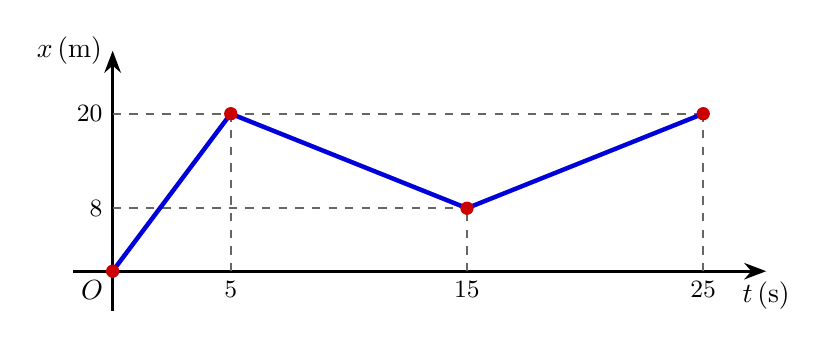
\begin{tikzpicture}[>=Stealth, scale=1.0]
    % محورها
    \draw[->, line width=1.1pt] (-0.5,0) -- (8.3,0) node[below] {$t\,(\text{s})$};
    \draw[->, line width=1.1pt] (0,-0.5) -- (0,2.8) node[left] {$x\,(\text{m})$};
    \node[below left] at (0,0) {$O$};

    % خطوط راهنما
    \draw[dashed, line width=0.7pt, gray!80!black] (0,2) node[left, black] {\small $20$} -- (7.5,2);
    \draw[dashed, line width=0.7pt, gray!80!black] (0,0.8) node[left, black] {\small $8$} -- (4.5,0.8);
    \draw[dashed, line width=0.7pt, gray!80!black] (1.5,0) node[below, black] {\small $5$} -- (1.5,2);
    \draw[dashed, line width=0.7pt, gray!80!black] (4.5,0) node[below, black] {\small $15$} -- (4.5,0.8);
    \draw[dashed, line width=0.7pt, gray!80!black] (7.5,0) node[below, black] {\small $25$} -- (7.5,2);

    % نمودار چندبخشی
    \draw[line width=1.6pt, blue!85!black] (0,0) -- (1.5,2);
    \draw[line width=1.6pt, blue!85!black] (1.5,2) -- (4.5,0.8);
    \draw[line width=1.6pt, blue!85!black] (4.5,0.8) -- (7.5,2);

    % نقاط کلیدی
    \filldraw[red!80!black] (0,0) circle (2.2pt);
    \filldraw[red!80!black] (1.5,2) circle (2.2pt);
    \filldraw[red!80!black] (4.5,0.8) circle (2.2pt);
    \filldraw[red!80!black] (7.5,2) circle (2.2pt);
\end{tikzpicture}
\end{center}

\begin{enumerate}
    \item[الف)] بیشترین فاصلهٔ متحرک از مبدأ مکان چند متر است؟
    \item[ب)] متحرک در کدام بازهٔ زمانی در خلاف جهت محور $x$ حرکت می‌کند؟
    \item[پ)] مسافت پیموده‌شده توسط متحرک در بازهٔ زمانی $0$ تا $25\,\text{s}$ را به دست آورید.
    \item[ت)] اندازهٔ سرعت متوسط متحرک در بازهٔ زمانی $5\,\text{s}$ تا $25\,\text{s}$ چقدر است؟
\end{enumerate}
\end{exambox}

\begin{answerbox}{پاسخ تشریحی سوال ۱}

\begin{itemize}
    \item[الف)] بیشترین فاصله از مبدأ، بیشترین مقدار قدرمطلق مکان است. با توجه به نمودار، بزرگ‌ترین مقدار مکان برابر است با:
    \[
    x_{\max} = 20\,\text{m}
    \]

    \item[ب)] حرکت در خلاف جهت محور $x$ یعنی سرعت منفی؛ یعنی بخشی از نمودار که شیب منفی (نزولی) دارد:
    \[
    \text{\rl{بازهٔ زمانی:}} \quad [5\,\text{s}, 15\,\text{s}]
    \]

    \item[پ)] چون متحرک یک بار تغییر جهت داده است، مسافت را مرحله‌به‌مرحله محاسبه می‌کنیم:
    \begin{itemize}
        \item مرحلهٔ اول ($0$ تا $5\,\text{s}$): از $x=0$ تا $x=20\,\text{m}$ $\Rightarrow \ell_1 = 20\,\text{m}$
        \item مرحلهٔ دوم ($5\,\text{s}$ تا $15\,\text{s}$): برگشت از $x=20\,\text{m}$ تا $x=8\,\text{m}$ $\Rightarrow \ell_2 = 12\,\text{m}$
        \item مرحلهٔ سوم ($15\,\text{s}$ تا $25\,\text{s}$): از $x=8\,\text{m}$ تا $x=20\,\text{m}$ $\Rightarrow \ell_3 = 12\,\text{m}$
    \end{itemize}
    \[
    \ell = \ell_1 + \ell_2 + \ell_3 = 20 + 12 + 12 = 44\,\text{m}
    \]

    \item[ت)] مکان متحرک در ابتدا و انتهای این بازه برابر است ($x(5) = x(25) = 20\,\text{m}$)؛ بنابراین:
    \[
    \Delta x = x(25) - x(5) = 20 - 20 = 0 \quad \Longrightarrow \quad |\vec{v}_{av}| = \frac{|\Delta x|}{\Delta t} = \frac{0}{20} = 0
    \]
    توجه کنید که اگر تندی متوسط خواسته می‌شد، پاسخ صفر نمی‌شد؛ بلکه $s_{av} = \dfrac{24}{20} = 1.2\,\text{m/s}$ به دست می‌آمد.
\end{itemize}
\end{answerbox}

\vspace{0.3cm}

% --- سوال ۲ ---
\begin{exambox}{سوال ۲: معادلهٔ مکان-زمان و دیدار دو خودرو}
دو خودرو $A$ و $B$ که روی خط راست و در راستای محور $x$ حرکت می‌کنند، در لحظهٔ $t=0$ به ترتیب در مکان‌های $10\,\text{m}$ و $85\,\text{m}$ قرار دارند. خودروی $A$ با سرعت ثابت $+5\,\text{m/s}$ و خودروی $B$ با سرعت ثابت $-10\,\text{m/s}$ حرکت می‌کنند.

\begin{enumerate}
    \item[الف)] معادلهٔ مکان-زمان حرکت هر خودرو را بنویسید.
    \item[ب)] تعیین کنید خودروها در چه لحظه‌ای و در چه مکانی از کنار یکدیگر می‌گذرند.
    \item[پ)] با رسم نمودار مکان-زمان هر دو خودرو در یک دستگاه مختصات، نتیجهٔ قسمت «ب» را بررسی کنید.
\end{enumerate}
\end{exambox}

\begin{answerbox}{پاسخ تشریحی سوال ۲}

\begin{itemize}
    \item[الف)] با جای‌گذاری $x_0$ و $v$ هر خودرو در معادلهٔ ۱-۴:
    \[
    x_A = 5t + 10 \qquad , \qquad x_B = -10t + 85 \qquad \text{\rl{(برحسب SI)}}
    \]

    \item[ب)] در لحظهٔ گذر از کنار یکدیگر، مکان دو خودرو برابر است:
    \[
    5t + 10 = -10t + 85 \quad \Longrightarrow \quad 15t = 75 \quad \Longrightarrow \quad t = 5\,\text{s}
    \]
    \[
    x_A = 5(5) + 10 = 35\,\text{m} \qquad , \qquad x_B = -10(5) + 85 = 35\,\text{m}
    \]
    پس دو خودرو پس از $5\,\text{s}$ در مکان $x = 35\,\text{m}$ به یکدیگر می‌رسند.

    \item[پ)]
\end{itemize}

\begin{center}
\begin{tikzpicture}[>=Stealth, scale=1.0]
    % محورها
    \draw[->, line width=1.1pt] (-0.4,0) -- (5.2,0) node[below] {$t\,(\text{s})$};
    \draw[->, line width=1.1pt] (0,-0.4) -- (0,4.7) node[left] {$x\,(\text{m})$};
    \node[below left] at (0,0) {$O$};

    % مقادیر محور قائم
    \node[left, black] at (0,0.5) {\small $10$};
    \node[left, black] at (0,1.75) {\small $35$};
    \node[left, black] at (0,4.25) {\small $85$};

    % خطوط حرکت
    \draw[line width=1.5pt, blue!85!black] (0,0.5) -- (4.4,2.5) node[right, black] {$A$};
    \draw[line width=1.5pt, red!80!black] (0,4.25) -- (4.4,0.25) node[right, black] {$B$};

    % نقطه دیدار
    \draw[dashed, line width=0.7pt, gray!80!black] (0,1.75) -- (2.75,1.75) -- (2.75,0);
    \node[below, black] at (2.75,0) {\small $5$};
    \filldraw[purple] (2.75,1.75) circle (2.6pt);
    \node[above right=1pt, purple] at (2.75,1.75) {\small\rl{دیدار}};
\end{tikzpicture}
\end{center}

محل تقاطع دو خط دقیقاً نقطهٔ $(5\,\text{s}, 35\,\text{m})$ است که با حل جبری قسمت «ب» نیز به دست آمد.
\end{answerbox}

\vspace{0.3cm}

% --- سوال ۳ ---
\begin{exambox}{سوال ۳: تحلیل نمودار سرعت-زمان}
نمودار سرعت-زمان خودرویی که در راستای محور $x$ حرکت می‌کند، مطابق شکل زیر است:

\begin{center}
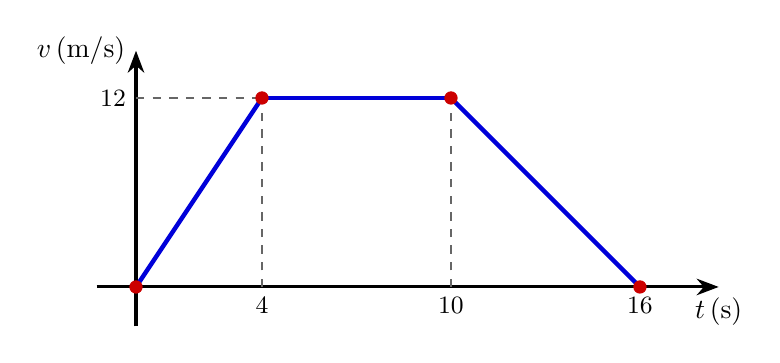
\begin{tikzpicture}[>=Stealth, scale=1.0]
    % محورها
    \draw[->, line width=1.1pt] (-0.5,0) -- (7.4,0) node[below] {$t\,(\text{s})$};
    \draw[->, line width=1.1pt] (0,-0.5) -- (0,3) node[left] {$v\,(\text{m/s})$};

    % خطوط راهنما
    \draw[dashed, line width=0.7pt, gray!80!black] (0,2.4) node[left, black] {\small $12$} -- (4,2.4);
    \draw[dashed, line width=0.7pt, gray!80!black] (1.6,0) node[below, black] {\small $4$} -- (1.6,2.4);
    \draw[dashed, line width=0.7pt, gray!80!black] (4,0) node[below, black] {\small $10$} -- (4,2.4);
    \draw[dashed, line width=0.7pt, gray!80!black] (6.4,0) node[below, black] {\small $16$} -- (6.4,0);

    % نمودار
    \draw[line width=1.6pt, blue!85!black] (0,0) -- (1.6,2.4);
    \draw[line width=1.6pt, blue!85!black] (1.6,2.4) -- (4,2.4);
    \draw[line width=1.6pt, blue!85!black] (4,2.4) -- (6.4,0);

    % نقاط کلیدی
    \filldraw[red!80!black] (0,0) circle (2.2pt);
    \filldraw[red!80!black] (1.6,2.4) circle (2.2pt);
    \filldraw[red!80!black] (4,2.4) circle (2.2pt);
    \filldraw[red!80!black] (6.4,0) circle (2.2pt);
\end{tikzpicture}
\end{center}

\begin{enumerate}
    \item[الف)] شتاب خودرو را در هر یک از سه بازهٔ زمانی به دست آورید.
    \item[ب)] جابه‌جایی خودرو در کل زمان حرکت ($16\,\text{s}$) را با محاسبهٔ مساحت زیر نمودار بیابید.
    \item[پ)] معادلهٔ سرعت-زمان خودرو را در بازهٔ زمانی $0$ تا $4\,\text{s}$ بنویسید.
    \item[ت)] آیا در این حرکت، مسافت پیموده‌شده با جابه‌جایی برابر است؟ چرا؟
    \item[ث)] نمودار شتاب-زمان خودرو را در بازهٔ زمانی $0$ تا $16\,\text{s}$ رسم کنید.
\end{enumerate}
\end{exambox}

\begin{answerbox}{پاسخ تشریحی سوال ۳}

\begin{itemize}
    \item[الف)] شتاب در هر بازه برابر شیب نمودار در آن بازه است:
    \[
    a_{[0,4]} = \frac{12-0}{4-0} = +3\,\frac{\text{m}}{\text{s}^2}
    \qquad , \qquad
    a_{[4,10]} = 0
    \qquad , \qquad
    a_{[10,16]} = \frac{0-12}{16-10} = -2\,\frac{\text{m}}{\text{s}^2}
    \]

    \item[ب)] جابه‌جایی برابر مساحت ناحیهٔ زیر نمودار (تراپز) است:
    \[
    \Delta x = \underbrace{\frac{1}{2}(4)(12)}_{24} + \underbrace{(6)(12)}_{72} + \underbrace{\frac{1}{2}(6)(12)}_{36} = 132\,\text{m}
    \]

    \item[پ)] در بازهٔ اول $v_0 = 0$ و $a = 3\,\text{m/s}^2$ است؛ پس از معادلهٔ ۱-۸:
    \[
    v = at + v_0 \quad \Longrightarrow \quad v = 3t \qquad \text{\rl{(برحسب SI)}}
    \]

    \item[ت)] بله؛ زیرا سرعت خودرو در تمام طول حرکت نامنفی است ($v \ge 0$)، نمودار هیچ گاه از محور زمان پایین نمی‌رود و در نتیجه همهٔ نواحی زیر نمودار مثبت‌اند. پس $\ell = \Delta x = 132\,\text{m}$.

    \item[ث)] شتاب در هر بازه ثابت است (قسمت «الف»)؛ بنابراین نمودار شتاب-زمان، نموداری پله‌ای با سه سطح افقی است:
    \begin{center}
    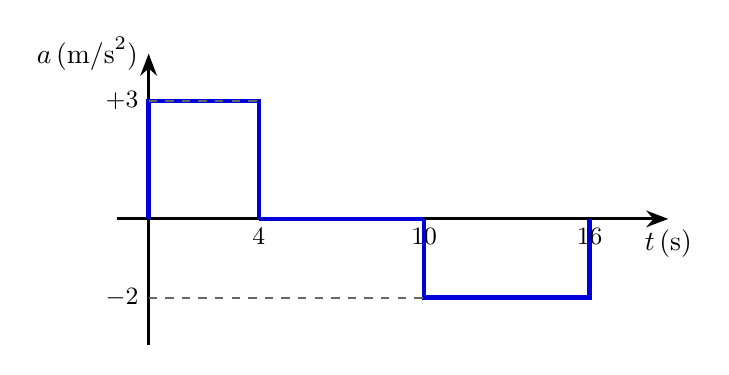
\begin{tikzpicture}[>=Stealth, scale=1.0]
        % محورها
        \draw[->, line width=1.1pt] (-0.4,0) -- (6.6,0) node[below] {$t\,(\text{s})$};
        \draw[->, line width=1.1pt] (0,-1.6) -- (0,2.1) node[left] {$a\,(\text{m/s}^2)$};

        % نمودار پله‌ای
        \draw[line width=1.6pt, blue!85!black] (0,0) -- (0,1.5) -- (1.4,1.5) -- (1.4,0)
              (1.4,0) -- (3.5,0)
              (3.5,0) -- (3.5,-1.0) -- (5.6,-1.0) -- (5.6,0);

        % خطوط راهنما و برچسب‌ها
        \draw[dashed, line width=0.7pt, gray!80!black] (0,1.5) node[left, black] {\small $+3$} -- (1.4,1.5);
        \draw[dashed, line width=0.7pt, gray!80!black] (0,-1.0) node[left, black] {\small $-2$} -- (3.5,-1.0);
        \foreach \x/\l in {1.4/{4}, 3.5/{10}, 5.6/{16}} {
            \node[below, black] at (\x,0) {\small \l};
        }
    \end{tikzpicture}
    \end{center}
    وارسی مفید: مساحت سطح بین این نمودار و محور زمان برابر $(3)(4) + (0)(6) + (-2)(6) = 12 - 12 = 0$ است؛ یعنی تغییر سرعت کل صفر است و این با برابری سرعت اولیه و انتهای حرکت ($0$ و $0$) سازگار است.
\end{itemize}
\end{answerbox}

\vspace{0.3cm}

% --- سوال ۴ ---
\begin{exambox}{سوال ۴: مسئلهٔ ترمز و مسئلهٔ تعقیب (حرکت با شتاب ثابت)}
\textbf{الف)} خودرویی با سرعت $72\,\text{km/h}$ در حال حرکت روی خط راست است که ناگهان راننده ترمز می‌گیرد و خودرو با شتاب ثابت $4\,\text{m/s}^2$ کند می‌شود تا بایستد. فاصلهٔ طی‌شده تا توقف کامل و مدت زمان ترمزگیری را بیابید.

\vspace{0.25cm}
\textbf{ب)} موتورسیکلتی از حال سکون و با شتاب ثابت $3\,\text{m/s}^2$ شروع به حرکت می‌کند؛ دقیقاً در همین لحظه خودرویی با سرعت ثابت $30\,\text{m/s}$ از کنار او عبور می‌کند و در همان جهت ادامه می‌دهد. موتورسیکلت در چه لحظه‌ای و در چه مکانی به خودرو می‌رسد؟
\end{exambox}

\begin{answerbox}{پاسخ تشریحی سوال ۴}
\textbf{قسمت الف)} ابتدا یکاها را هماهنگ می‌کنیم:
\[
v_0 = \frac{72}{3.6} = 20\,\frac{\text{m}}{\text{s}} \qquad , \qquad v = 0 \qquad , \qquad a = -4\,\frac{\text{m}}{\text{s}^2}
\]
چون زمان داده نشده است، از معادلهٔ ۱-۱۱ استفاده می‌کنیم:
\[
v^2 = v_0^2 + 2a\,\Delta x \quad \Longrightarrow \quad 0 = (20)^2 + 2(-4)\,\Delta x \quad \Longrightarrow \quad \Delta x = \frac{400}{8} = 50\,\text{m}
\]
و از معادلهٔ ۱-۸ برای زمان توقف:
\[
v = at + v_0 \quad \Longrightarrow \quad 0 = (-4)t + 20 \quad \Longrightarrow \quad t = 5\,\text{s}
\]

\vspace{0.25cm}
\textbf{قسمت ب)} مبدأ مکان را محل عبور خودرو در لحظهٔ $t=0$ می‌گیریم. معادلهٔ مکان-زمان هر متحرک را می‌نویسیم:
\[
x_{\text{\rl{خودرو}}} = 30t \qquad , \qquad x_{\text{\rl{موتور}}} = \frac{1}{2}(3)t^2 = 1.5t^2
\]
در لحظهٔ رسیدن، مکان دو وسیله برابر است:
\[
1.5t^2 = 30t \quad \Longrightarrow \quad t(1.5t - 30) = 0
\]
جواب $t=0$ همان لحظهٔ عبور اولیه است؛ جواب قابل قبول:
\[
t = 20\,\text{s} \qquad , \qquad x = 30(20) = 600\,\text{m}
\]
بنابراین موتورسیکلت پس از $20\,\text{s}$ و در فاصلهٔ $600\,\text{m}$ از نقطهٔ شروع به خودرو می‌رسد.
\end{answerbox}

\vspace{0.3cm}

% --- سوال ۵ ---
\begin{exambox}{سوال ۵: سقوط آزاد}
سنگی را از بام ساختمانی بدون سرعت اولیه رها می‌کنند و سنگ با تندی $39.2\,\text{m/s}$ به زمین برخورد می‌کند. (مقاومت هوا را ناچیز بگیرید و $g = 9.8\,\text{m/s}^2$.)

\begin{enumerate}
    \item[الف)] مدت زمان سقوط سنگ چقدر است؟
    \item[ب)] ارتفاع ساختمان چند متر است؟
    \item[پ)] سنگ در ثانیهٔ آخر سقوط خود چند متر را طی کرده است؟
\end{enumerate}
\end{exambox}

\begin{answerbox}{پاسخ تشریحی سوال ۵}

جهت رو به بالا را مثبت می‌گیریم و مبدأ مکان را بام ساختمان در نظر می‌گیریم؛ پس $y_0 = 0$، $v_0 = 0$ و سطح زمین در $y = -h$ قرار دارد.

\begin{itemize}
    \item[الف)] از معادلهٔ $v = -gt$:
    \[
    -39.2 = -(9.8)t \quad \Longrightarrow \quad t = 4\,\text{s}
    \]

    \item[ب)] از معادلهٔ $y = -\frac{1}{2}gt^2$ در لحظهٔ برخورد:
    \[
    -h = -\frac{1}{2}(9.8)(4)^2 \quad \Longrightarrow \quad h = 78.4\,\text{m}
    \]

    \item[پ)] ابتدا مکان سنگ را در پایان ثانیهٔ سوم می‌یابیم:
    \[
    y(3) = -\frac{1}{2}(9.8)(3)^2 = -44.1\,\text{m}
    \]
    مسافت طی‌شده در ثانیهٔ آخر (از $t=3\,\text{s}$ تا $t=4\,\text{s}$):
    \[
    d = |y(4) - y(3)| = |-78.4 - (-44.1)| = 34.3\,\text{m}
    \]
\end{itemize}
\end{answerbox}

% =========================================================================
% بخش ۷: بانک تست‌های چهارگزینه‌ای کنکور
% =========================================================================
\section{بانک تست‌های چهارگزینه‌ای کنکور}

تست‌های زیر به سبک سوالات آزمون سراسری طراحی شده‌اند و هر کدام بر یکی از \textbf{تله‌های رایج} این فصل تمرکز دارند. توصیه می‌کنیم مانند روز آزمون، برای هر تست حدود یک دقیقه و نیم زمان بگذارید و سپس پاسخ تشریحی را مطالعه کنید.

% --- تست ۱ ---
\begin{exambox}{تست ۱: مسافت، جابه‌جایی، تندی متوسط و سرعت متوسط}
دونده‌ای روی خط راست حرکت می‌کند؛ او از مبدأ مکان شروع کرده، $100\,\text{m}$ در جهت مثبت محور $x$ می‌دود، بی‌درنگ بازمی‌گردد و $40\,\text{m}$ در جهت مخالف می‌دود. اگر کل حرکت او $20\,\text{s}$ طول بکشد، نسبت تندی متوسط به اندازهٔ سرعت متوسط او چقدر است؟

\begin{center}
\begin{tabular}{p{7cm} p{7cm}}
۱) $\dfrac{7}{3}$ & ۲) $\dfrac{3}{7}$ \\[0.35cm]
۳) $\dfrac{5}{2}$ & ۴) $1$ \\
\end{tabular}
\end{center}
\end{exambox}

\begin{answerbox}{پاسخ تست ۱}

\textbf{پاسخ: گزینهٔ ۱}

\textbf{تشریح:} مسافت پیموده‌شده و جابه‌جایی دونده را جداگانه محاسبه می‌کنیم:
\[
\ell = 100 + 40 = 140\,\text{m}
\qquad , \qquad
\Delta x = 100 - 40 = 60\,\text{m}
\]
بنابراین:
\[
s_{av} = \frac{\ell}{\Delta t} = \frac{140}{20} = 7\,\frac{\text{m}}{\text{s}}
\qquad , \qquad
|\vec{v}_{av}| = \frac{|\Delta x|}{\Delta t} = \frac{60}{20} = 3\,\frac{\text{m}}{\text{s}}
\quad \Longrightarrow \quad \frac{s_{av}}{|\vec{v}_{av}|} = \frac{7}{3}
\]

\textbf{تحلیل تله:} داوطلبی که جابه‌جایی را با مسافت اشتباه بگیرد ($\Delta x = 140$)، به نسبت $1$ یعنی گزینهٔ ۴ می‌رسد؛ این دقیقاً همان تلهٔ طراح است.
\end{answerbox}

\vspace{0.25cm}

% --- تست ۲ ---
\begin{exambox}{تست ۲: شرط برابری تندی متوسط و اندازهٔ سرعت متوسط (مفهومی)}
در کدام حالت، تندی متوسط با اندازهٔ سرعت متوسط برابر است؟

\begin{center}
\begin{tabular}{p{15cm}}
۱) در هر حرکت مستقیم‌الخط، حتی اگر متحرک تغییر جهت دهد \\
[0.2cm] ۲) تنها در حرکت با سرعت ثابت \\
[0.2cm] ۳) در حرکت روی خط راست، مشروط بر آنکه متحرک در طول حرکت تغییر جهت ندهد \\
[0.2cm] ۴) در هیچ حرکتی این دو کمیت با هم برابر نمی‌شوند \\
\end{tabular}
\end{center}
\end{exambox}

\begin{answerbox}{پاسخ تست ۲}

\textbf{پاسخ: گزینهٔ ۳}

\textbf{تشریح:} چون همواره $\ell \ge |\Delta x|$ برقرار است، دو کمیت تنها زمانی برابرند که $\ell = |\Delta x|$ باشد؛ یعنی متحرک روی خط راست حرکت کند و هیچ‌گاه تغییر جهت ندهد.

\textbf{تحلیل تله:} گزینهٔ ۱ فراموش می‌کند که در حرکت مستقیم‌الخط با بازگشت، مسافت از اندازهٔ جابه‌جایی بیشتر می‌شود. گزینهٔ ۲ شرط را بیش از حد محدود می‌کند؛ حرکت با شتاب ثابت روی خط راست بدون تغییر جهت نیز این برابری را دارد.
\end{answerbox}

\vspace{0.25cm}

% --- تست ۳ ---
\begin{exambox}{تست ۳: لحظهٔ توقف از روی معادلهٔ مکان-زمان}
متحرکی روی خط راست با معادلهٔ مکان-زمان $x = t^2 - 4t + 6$ (برحسب SI) در حال حرکت است. متحرک در چه لحظه‌ای موقتاً می‌ایستد؟

\begin{center}
\begin{tabular}{p{7cm} p{7cm}}
۱) $t = 1\,\text{s}$ & ۲) $t = 2\,\text{s}$ \\[0.35cm]
۳) $t = 4\,\text{s}$ & ۴) $t = 6\,\text{s}$ \\
\end{tabular}
\end{center}
\end{exambox}

\begin{answerbox}{پاسخ تست ۳}

\textbf{پاسخ: گزینهٔ ۲}

\textbf{تشریح:} توقف لحظه‌ای یعنی سرعت لحظه‌ای صفر است. چون مکان متحرک تابعی درجه دوم از زمان است (حرکت با شتاب ثابت)، سرعت از رابطهٔ ۱-۸ با $v_0 = -4\,\text{m/s}$ و $a = 2\,\text{m/s}^2$ به دست می‌آید:
\[
v = at + v_0 = 2t - 4
\]
با قراردادن $v = 0$:
\[
2t - 4 = 0 \quad \Longrightarrow \quad t = 2\,\text{s}
\]

\textbf{تحلیل تله:} برخی داوطلبان به اشتباه معادلهٔ \textbf{مکان} را صفر قرار می‌دهند ($x=0$ یعنی عبور از مبدأ مکان، نه توقف!). توقف همیشه یعنی $v=0$. همچنین توجه کنید که پاسخ باید از شیب نمودار مکان-زمان (سرعت) به دست آید، نه از خود مکان.
\end{answerbox}

\vspace{0.25cm}

% --- تست ۴ ---
\begin{exambox}{تست ۴: جابه‌جایی و مسافت از روی نمودار $v$-$t$}
نمودار سرعت-زمان متحرکی روی خط راست، خط راستی است که از نقطهٔ $(0, +8\,\text{m/s})$ شروع شده و در لحظهٔ $t = 4\,\text{s}$ به $-8\,\text{m/s}$ می‌رسد. جابه‌جایی و مسافت متحرک در این بازهٔ زمانی به ترتیب کدام است؟

\begin{center}
\begin{tabular}{p{7cm} p{7cm}}
۱) صفر و صفر & ۲) صفر و $16\,\text{m}$ \\[0.35cm]
۳) $16\,\text{m}$ و صفر & ۴) $32\,\text{m}$ و $32\,\text{m}$ \\
\end{tabular}
\end{center}
\end{exambox}

\begin{answerbox}{پاسخ تست ۴}

\textbf{پاسخ: گزینهٔ ۲}

\textbf{تشریح:} جابه‌جایی برابر مساحت جبری زیر نمودار است. چون نمودار خطی است، از میانگین سرعت ابتدا و انتها (معادلهٔ ۱-۹) استفاده می‌کنیم:
\[
\Delta x = v_{av}\,\Delta t = \left(\frac{8 + (-8)}{2}\right)(4) = 0
\]
برای مسافت، نواحی بالا و پایین محور زمان را جدا می‌کنیم. نمودار در وسط بازه ($t = 2\,\text{s}$) محور زمان را قطع می‌کند:
\[
\ell = \underbrace{\frac{1}{2}(2)(8)}_{\text{\rl{بالا}}} + \underbrace{\frac{1}{2}(2)(8)}_{\text{\rl{پایین}}} = 8 + 8 = 16\,\text{m}
\]

\textbf{تحلیل تله:} اگر نواحی زیر محور زمان را نیز مثبت حساب کنید (نادیده گرفتن علامت)، به گزینهٔ ۴ می‌رسید. مساحت زیر محور زمان همواره \textbf{منفی} است.
\end{answerbox}

\vspace{0.25cm}

% --- تست ۵ ---
\begin{exambox}{تست ۵: تشخیص نوع حرکت از علامت سرعت و شتاب}
اگر در حرکت روی خط راست، سرعت متحرکی منفی و شتاب آن مثبت باشد، حرکت متحرک ... .

\begin{center}
\begin{tabular}{p{7cm} p{7cm}}
۱) تندشونده است & ۲) کندشونده است \\[0.35cm]
۳) با سرعت ثابت است & ۴) ابتدا کندشونده و سپس تندشونده است \\
\end{tabular}
\end{center}
\end{exambox}

\begin{answerbox}{پاسخ تست ۵}

\textbf{پاسخ: گزینهٔ ۲}

\textbf{تشریح:} قاعدهٔ تصمیم‌گیری، هم‌جهتی یا خلاف‌جهتی سرعت و شتاب است. سرعت منفی یعنی حرکت در جهت منفی محور $x$ و شتاب مثبت یعنی جهت شتاب در جهت مثبت محور است؛ پس سرعت و شتاب \textbf{خلاف جهت} یکدیگرند و تندی متحرک کاهش می‌یابد؛ بنابراین حرکت کندشونده است.

\textbf{تحلیل تله:} تصور رایج و غلط این است که «شتاب مثبت یعنی تندشونده». علامت شتاب تنها جهت آن را نسبت به محور مشخص می‌کند؛ آنچه نوع حرکت را تعیین می‌کند، مقایسهٔ جهت شتاب با جهت سرعت است.
\end{answerbox}

\vspace{0.25cm}

% --- تست ۶ ---
\begin{exambox}{تست ۶: نسبت‌های سقوط آزاد}
جسمی را بدون سرعت اولیه و با چشم‌پوشی از مقاومت هوا رها می‌کنیم. نسبت مسافتی که جسم در \textbf{ثانیهٔ سوم} سقوط می‌پیماید به کل مسافت طی‌شده در سه ثانیهٔ اول چقدر است؟

\begin{center}
\begin{tabular}{p{7cm} p{7cm}}
۱) $\dfrac{5}{9}$ & ۲) $\dfrac{1}{3}$ \\[0.35cm]
۳) $\dfrac{1}{9}$ & ۴) $\dfrac{5}{7}$ \\
\end{tabular}
\end{center}
\end{exambox}

\begin{answerbox}{پاسخ تست ۶}

\textbf{پاسخ: گزینهٔ ۱}

\textbf{تشریح:} در سقوط آزاد بدون سرعت اولیه، مسافت طی‌شده در ثانیه‌های متوالی اول، دوم و سوم به ترتیب متناسب با اعداد فرد $1$، $3$ و $5$ است (زیرا $y_n - y_{n-1} \propto (2n-1)$). پس:
\[
d_1 : d_2 : d_3 = 1 : 3 : 5 \quad \Longrightarrow \quad d_3 = 5k \; , \; d_{\text{\rl{کل}}} = 1k + 3k + 5k = 9k
\]
\[
\frac{d_3}{d_{\text{\rl{کل}}}} = \frac{5}{9}
\]
برای وارسی، با $g = 10\,\text{m/s}^2$: مسافت ثانیهٔ سوم برابر است با $\frac{1}{2}(10)(9) - \frac{1}{2}(10)(4) = 45 - 20 = 25\,\text{m}$ و کل مسافت $\frac{1}{2}(10)(9) = 45\,\text{m}$؛ نسبت برابر $\frac{25}{45} = \frac{5}{9}$ است.

\textbf{تحلیل تله:} گزینهٔ ۲ تلهٔ «مسافت ثانیهٔ سوم به مسافت دو ثانیهٔ اول» نیست بلکه نسبت سادهٔ زمان‌هاست؛ و گزینهٔ ۳ نسبت مسافت ثانیهٔ اول به کل است. دقت کنید که «در ثانیهٔ سوم» با «تا پایان ثانیهٔ سوم» تفاوت اساسی دارد.
\end{answerbox}

% =========================================================================
% بخش ۸: جمع‌بندی نهایی فصل
% =========================================================================
\section{جمع‌بندی نهایی فصل}

\begin{summarybox}{نقشهٔ یک‌نگاهی فرمول‌های فصل (سیستم ذهنی)}
نقشهٔ زیر تمام روابط فصل را بر پایهٔ دسته‌بندی موضوعی در یک نگاه نشان می‌دهد. پیش از امتحان، سعی کنید آن را بدون نگاه کردن در ذهن خود بازسازی کنید؛ هر گره‌ای که فراموش شد، نشان‌دهندهٔ بخشی است که باید دوباره مرور شود:
\begin{center}
\begin{tikzpicture}[>=Stealth]
    \tikzset{
        fmap chip/.style={anchor=east, font=\small, rounded corners=2.2pt, line width=0.6pt, inner sep=3.2pt},
        leafA/.style={fmap chip, draw=teal!60!black, fill=teal!7},
        leafB/.style={fmap chip, draw=blue!60!black, fill=blue!7},
        leafC/.style={fmap chip, draw=orange!80!black, fill=orange!9},
        leafD/.style={fmap chip, draw=red!60!black, fill=red!7},
        leafE/.style={fmap chip, draw=violet!65!black, fill=violet!7},
        fmap group/.style={anchor=center, rounded corners=3pt, line width=0.9pt, font=\footnotesize\bfseries, align=center, inner sep=4.5pt, text width=2.05cm, text=white},
        grpA/.style={fmap group, draw=teal!85!black, fill=teal!70!black},
        grpB/.style={fmap group, draw=blue!85!black, fill=blue!70!black},
        grpC/.style={fmap group, draw=orange!90!black, fill=orange!80!black},
        grpD/.style={fmap group, draw=red!80!black, fill=red!70!black},
        grpE/.style={fmap group, draw=violet!85!black, fill=violet!75!black},
        fmap root/.style={anchor=center, rounded corners=4pt, line width=1.3pt, font=\footnotesize\bfseries, align=center, inner sep=6pt, text width=1.6cm, minimum height=1.05cm, text=white, draw=purple!85!black, fill=purple!75!black},
        zone/.style={rounded corners=7pt, inner sep=6.5pt, line width=0.5pt},
        zoneA/.style={zone, draw=teal!30, fill=teal!4},
        zoneB/.style={zone, draw=blue!30, fill=blue!4},
        zoneC/.style={zone, draw=orange!35, fill=orange!5},
        zoneD/.style={zone, draw=red!30, fill=red!4},
        zoneE/.style={zone, draw=violet!30, fill=violet!4},
        fmap arrow/.style={->, line width=0.65pt},
        arrA/.style={fmap arrow, teal!70!black},
        arrB/.style={fmap arrow, blue!70!black},
        arrC/.style={fmap arrow, orange!90!black},
        arrD/.style={fmap arrow, red!70!black},
        arrE/.style={fmap arrow, violet!75!black},
        trunk/.style={->, line width=0.9pt}
    }
    % ---------- گروه پارامترهای حرکت ----------
    \node[leafA] (A1) at (4.7, 0)    {\lr{$s_{av} = \frac{\ell}{\Delta t}$} \rl{تندی متوسط:} \textcolor{teal!70!black}{\footnotesize$\bullet$}};
    \node[leafA] (A2) at (4.7, -0.7) {\lr{$v_{av} = \frac{\Delta x}{\Delta t}$} \rl{سرعت متوسط:} \textcolor{teal!70!black}{\footnotesize$\bullet$}};
    \node[leafA] (A3) at (4.7, -1.4) {\lr{$a_{av} = \frac{\Delta v}{\Delta t}$} \rl{شتاب متوسط:} \textcolor{teal!70!black}{\footnotesize$\bullet$}};
    \node[grpA] (grpA) at (7.2, -0.7) {\rl{پارامترهای حرکت}};

    % ---------- گروه حرکت با سرعت ثابت ----------
    \node[leafB] (B1) at (4.7, -2.6) {\lr{$x = v\,t + x_0$} \rl{معادلهٔ مکان-زمان:} \textcolor{blue!70!black}{\footnotesize$\bullet$}};
    \node[grpB] (grpB) at (7.2, -2.6) {\rl{حرکت با سرعت ثابت}};

    % ---------- گروه حرکت با شتاب ثابت ----------
    \node[leafC] (C1) at (4.7, -3.75) {\lr{$v = a\,t + v_0$} \rl{معادلهٔ سرعت-زمان:} \textcolor{orange!90!black}{\footnotesize$\bullet$}};
    \node[leafC] (C2) at (4.7, -4.45) {\lr{$x = \frac{1}{2}a\,t^2 + v_0\,t + x_0$} \rl{معادلهٔ مکان-زمان:} \textcolor{orange!90!black}{\footnotesize$\bullet$}};
    \node[leafC] (C3) at (4.7, -5.15) {\lr{$v_{av} = \frac{v_1 + v_2}{2}$} \rl{معادلهٔ سرعت متوسط:} \textcolor{orange!90!black}{\footnotesize$\bullet$}};
    \node[leafC] (C4) at (4.7, -5.85) {\lr{$\Delta x = \frac{v_1 + v_2}{2}\,t$} \rl{مستقل از شتاب:} \textcolor{orange!90!black}{\footnotesize$\bullet$}};
    \node[leafC] (C5) at (4.7, -6.55) {\lr{$v_2^2 - v_1^2 = 2a\,\Delta x$} \rl{مستقل از زمان:} \textcolor{orange!90!black}{\footnotesize$\bullet$}};
    \node[leafC] (C6) at (4.7, -7.25) {\lr{$\Delta x = -\frac{1}{2}a\,t^2 + v_2\,t$} \rl{مستقل از سرعت اولیه:} \textcolor{orange!90!black}{\footnotesize$\bullet$}};
    \node[leafC] (C7) at (4.7, -7.95) {\lr{$\Delta x_n = (n - \frac{1}{2})\,a + v_0$} \rl{جابه‌جایی ثانیهٔ $n$‌ام:} \textcolor{orange!90!black}{\footnotesize$\bullet$}};
    \node[grpC] (grpC) at (7.2, -5.85) {\rl{حرکت با شتاب ثابت}};

    % ---------- گروه ترمز با شتاب ثابت ----------
    \node[leafD] (D1) at (4.7, -9.1) {\lr{$d_s = \frac{v_0^2}{2|a|}$} \rl{مسافت توقف:} \textcolor{red!70!black}{\footnotesize$\bullet$}};
    \node[leafD] (D2) at (4.7, -9.8) {\lr{$t_s = \left|\frac{v_0}{a}\right|$} \rl{زمان توقف:} \textcolor{red!70!black}{\footnotesize$\bullet$}};
    \node[grpD] (grpD) at (7.2, -9.45) {\rl{ترمز با شتاب ثابت}};

    % ---------- گروه سقوط آزاد ----------
    \node[leafE] (E1) at (4.7, -10.95) {\lr{$v = -g\,t$} \rl{سرعت-زمان:} \textcolor{violet!75!black}{\footnotesize$\bullet$}};
    \node[leafE] (E2) at (4.7, -11.65) {\lr{$y = -\frac{1}{2}g\,t^2 + y_0$} \rl{مکان-زمان:} \textcolor{violet!75!black}{\footnotesize$\bullet$}};
    \node[leafE] (E3) at (4.7, -12.35) {\lr{$v^2 = -2g\,\Delta y$} \rl{مستقل از زمان:} \textcolor{violet!75!black}{\footnotesize$\bullet$}};
    \node[leafE] (E4) at (4.7, -13.05) {\lr{$\Delta y_n = -\frac{1}{2}g\,(2n-1)$} \rl{جابه‌جایی ثانیهٔ $n$‌ام:} \textcolor{violet!75!black}{\footnotesize$\bullet$}};
    \node[grpE] (grpE) at (7.2, -12.0) {\rl{سقوط آزاد (رها شدن)}};

    % ---------- نواحی پس‌زمینه و سایهٔ ریشه ----------
    \begin{scope}[on background layer]
        \node[zoneA, fit=(A1)(A2)(A3)(grpA)] {};
        \node[zoneB, fit=(B1)(grpB)] {};
        \node[zoneC, fit=(C1)(C2)(C3)(C4)(C5)(C6)(C7)(grpC)] {};
        \node[zoneD, fit=(D1)(D2)(grpD)] {};
        \node[zoneE, fit=(E1)(E2)(E3)(E4)(grpE)] {};
        \node[fmap root, draw=none, fill=black!20] at (10.28, -6.58) {};
    \end{scope}

    % ---------- ریشه ----------
    \node[fmap root] (root) at (10.2, -6.5) {\rl{حرکت‌شناسی}\\ \rl{فصل ۱}};

    % ---------- یال‌های برگ ----------
    \draw[arrA] (A1.east) -- (grpA.west);
    \draw[arrA] (A2.east) -- (grpA.west);
    \draw[arrA] (A3.east) -- (grpA.west);
    \draw[arrB] (B1.east) -- (grpB.west);
    \draw[arrC] (C1.east) -- (grpC.west);
    \draw[arrC] (C2.east) -- (grpC.west);
    \draw[arrC] (C3.east) -- (grpC.west);
    \draw[arrC] (C4.east) -- (grpC.west);
    \draw[arrC] (C5.east) -- (grpC.west);
    \draw[arrC] (C6.east) -- (grpC.west);
    \draw[arrC] (C7.east) -- (grpC.west);
    \draw[arrD] (D1.east) -- (grpD.west);
    \draw[arrD] (D2.east) -- (grpD.west);
    \draw[arrE] (E1.east) -- (grpE.west);
    \draw[arrE] (E2.east) -- (grpE.west);
    \draw[arrE] (E3.east) -- (grpE.west);
    \draw[arrE] (E4.east) -- (grpE.west);

    % ---------- تنه‌های منحنی تا ریشه ----------
    \draw[trunk, teal!70!black]   (grpA.east) to[out=0, in=140] (root.west);
    \draw[trunk, blue!70!black]   (grpB.east) to[out=0, in=160] (root.west);
    \draw[trunk, orange!90!black] (grpC.east) -- (root.west);
    \draw[trunk, red!70!black]    (grpD.east) to[out=0, in=200] (root.west);
    \draw[trunk, violet!75!black] (grpE.east) to[out=0, in=220] (root.west);
\end{tikzpicture}
\end{center}
\end{summarybox}

\begin{summarybox}{جدول فرمول‌های طلایی فصل اول}
\begin{center}
\begin{tabular}{p{1.6cm} p{5.6cm} p{6.4cm}}
\toprule
\textbf{رابطه} & \textbf{فرمول} & \textbf{شرط کاربرد} \\
\midrule
۱-۱ & $s_{av} = \dfrac{\ell}{\Delta t}$ & همیشه (تندی متوسط) \\
۱-۲ / ۱-۳ & $v_{av} = \dfrac{\Delta x}{\Delta t}$ & همیشه (سرعت متوسط روی محور $x$) \\
۱-۴ & $x = vt + x_0$ & فقط در حرکت با سرعت ثابت \\
۱-۵ / ۱-۶ & $a_{av} = \dfrac{v_2 - v_1}{t_2 - t_1}$ & همیشه (شتاب متوسط) \\
۱-۸ & $v = at + v_0$ & فقط در حرکت با شتاب ثابت \\
۱-۹ & $v_{av} = \dfrac{v + v_0}{2}$ & فقط در حرکت با شتاب ثابت \\
۱-۱۰ & $x = x_0 + v_0 t + \dfrac{1}{2}at^2$ & فقط در حرکت با شتاب ثابت \\
۱-۱۱ & $v^2 = v_0^2 + 2a\,\Delta x$ & فقط در حرکت با شتاب ثابت (بدون $t$) \\
ترکیبی & $\Delta x = \dfrac{v_1+v_2}{2}\,t$ & فقط در حرکت با شتاب ثابت (بدون $a$) \\
ثانیهٔ $n$‌ام & $\Delta x_n = \frac{1}{2}a\,(2n-1) + v_0$ & جابه‌جایی در ثانیهٔ $n$‌ام؛ شتاب ثابت \\
سقوط آزاد & $v = -gt$ ، $y = -\dfrac{1}{2}gt^2$ ، $v^2 = -2gy$ & بدون سرعت اولیه؛ جهت بالا مثبت \\
\bottomrule
\end{tabular}
\end{center}
\end{summarybox}

\begin{summarybox}{جدول تفسیر سه نمودار حیاتی فصل}
\begin{center}
\begin{tabular}{p{2.2cm} p{3.6cm} p{3.8cm} p{4cm}}
\toprule
\textbf{نمودار} & \textbf{شیب نشان می‌دهد} & \textbf{مساحت زیر نمودار} & \textbf{تقاطع با محور افقی} \\
\midrule
$x$-$t$ & سرعت (قاطع: متوسط، مماس: لحظه‌ای) & بی‌معنی & عبور از مبدأ مکان ($x=0$) \\
$v$-$t$ & شتاب & جابه‌جایی (با احتساب علامت) & تغییر جهت حرکت ($v=0$) \\
$a$-$t$ & — & تغییر سرعت ($\Delta v$) & سرعت ثابت ($a=0$) \\
\bottomrule
\end{tabular}
\end{center}
\end{summarybox}

\begin{summarybox}{ماتریس مقایسهٔ سه الگوی اصلی حرکت بر خط راست}
جدول زیر، سه الگوی اصلی حرکت این فصل را کنار هم قرار می‌دهد تا پیش از امتحان بتوانید با یک نگاه، تفاوت‌های کلیدی آن‌ها را مرور کنید:
\begin{center}
\begin{tabular}{p{2.4cm} p{3.4cm} p{4cm} p{4cm}}
\toprule
\textbf{ویژگی} & \textbf{حرکت یکنواخت} ($v=\text{cte}$) & \textbf{شتاب ثابت} ($a=\text{\rl{ثابت}}$) & \textbf{پرتاب قائم} ($a=-g$) \\
\midrule
شتاب & $a=0$ & $a \neq 0$ (ثابت) & $a=-g$ \\
معادلهٔ سرعت & $v = v_0 = \text{cte}$ & $v = at + v_0$ & $v = -gt + v_0$ \\
معادلهٔ مکان & $x = vt + x_0$ & $x = x_0 + v_0t + \frac{1}{2}at^2$ & $y = y_0 + v_0t - \frac{1}{2}gt^2$ \\
رابطهٔ بدون زمان & ندارد & $v^2 - v_0^2 = 2a\,\Delta x$ & $v^2 - v_0^2 = -2g\,\Delta y$ \\
نمودار $x$-$t$ & خط راست (شیب ثابت) & سهمی (تقعر به علامت $a$) & سهمی با تقعر رو به پایین \\
نمودار $v$-$t$ & خط افقی & خط راست با شیب $a$ & خط راست با شیب $-g$ \\
مساحت زیر $v$-$t$ & $\Delta x = v\,\Delta t$ & $\Delta x$ (ذوزنقه/مثلث) & $\Delta y$ (ذوزنقه/مثلث) \\
\bottomrule
\end{tabular}
\end{center}
توجه کنید که «سقوط بدون سرعت اولیه» حالت خاصی از ستون آخر است که در آن $v_0 = 0$ و مبدأ مکان، محل رها شدن جسم است.
\end{summarybox}

\begin{tipbox}{اشتباهات رایج - پیش از امتحان یک بار دیگر بخوانید}
\begin{enumerate}
    \item برابر گرفتن مسافت با اندازهٔ جابه‌جایی هنگامی که متحرک \textbf{تغییر جهت} داده است.
    \item استفاده از $v_{av} = \dfrac{v_1+v_2}{2}$ وقتی شتاب ثابت \textbf{نیست}؛ این رابطه فقط در حرکت با شتاب ثابت معتبر است.
    \item فراموش کردن علامت منفی شتاب در مسائل ترمز و کند شدن.
    \item جمع کردن مساحت‌های زیر نمودار $v$-$t$ بدون توجه به علامت نواحی پایین محور زمان.
    \item فراموش کردن تبدیل $\text{km/h}$ به $\text{m/s}$ (تقسیم بر $3.6$) پیش از جای‌گذاری در معادلات.
    \item در سقوط آزاد، مثبت گرفتن $g$ در حالی که جهت بالا را مثبت گرفته‌ایم؛ شتاب همواره $a = -g$ است.
    \item تصور اینکه $a > 0$ همیشه به معنای تندشونده بودن حرکت است؛ ملاک، هم‌جهتی سرعت و شتاب است.
    \item خواندن «مکان» به جای «فاصله از مبدأ»؛ فاصله از مبدأ برابر $|x|$ است نه خودِ $x$.
    \item اشتباه گرفتن «لحظهٔ توقف» ($v=0$) با «عبور از مبدأ مکان» ($x=0$).
\end{enumerate}
\end{tipbox}

\begin{summarybox}{سخن پایانی}
این جزوه همراه با بانک سوالات، تمام مفاهیم، معادلات و مهارت‌های نموداری مورد نیاز برای امتحان نهایی و کنکور را پوشش می‌دهد. توصیهٔ ما این است که پس از مطالعهٔ هر بخش، بدون نگاه به پاسخ‌ها سوالات مربوط به آن را حل کنید و تنها در گام آخر، حل خود را با پاسخ تشریحی مقایسه نمایید. موفق باشید.
\end{summarybox}

% =========================================================================
% [APPEND-POINT] ادامهٔ جزوه در بسته‌های بعدی پیش از این خط اضافه می‌شود
% =========================================================================

\end{document}
